% ------------------------------------------------------------------------
% MS Thesis of Nathaniel Enrique Eulin 
% Date Defended: May 1, 2025 
% ------------------------------------------------------------------------
\documentclass[letterpaper,12pt]{report}
\usepackage[centertags]{amsmath}
\usepackage{amsfonts}
\usepackage{amssymb}
\usepackage{amsthm}
\usepackage{newlfont}
\usepackage{epsfig}
\usepackage{UPCSTHESIS} %This loads the UP Computer Science Thesis Package
\usepackage{UPCSINC1}
\usepackage[active]{LTX}
\usepackage{subfigure}
\usepackage{listings}
\usepackage{array}
\usepackage{graphicx}
%\usepackage{float}
\usepackage{url}
\usepackage{lscape}

\usepackage{fancyhdr}

\fancyhf{} % clear all header and footer fields
\fancyhead[R]{\thepage}

\renewcommand{\headrulewidth}{0pt}
\renewcommand{\footrulewidth}{0pt}

% Redefining plain style which is automatically applied to chapters (including Bibliography)

\fancypagestyle{plain}{%
\fancyhf{} % clear all header and footer fields
\fancyhead[R]{\thepage}
\renewcommand{\headrulewidth}{0pt}
\renewcommand{\footrulewidth}{0pt}}

\pagestyle{fancy} 

%% Define a new 'leo' style for the package that will use a smaller font.
\makeatletter
\def\url@leostyle{%
  \@ifundefined{selectfont}{\def\UrlFont{\sf}}{\def\UrlFont{\small\ttfamily}}}
\makeatother
%% Now actually use the newly defined style.
\urlstyle{leo}


\hfuzz2pt
\newlength{\defbaselineskip}
\setlength{\defbaselineskip}{\baselineskip}
\newcommand{\setlinespacing}[1]%
           {\setlength{\baselineskip}{#1 \defbaselineskip}}
\newcommand{\doublespacing}{\setlength{\baselineskip}%
                           {2.0 \defbaselineskip}}
\newcommand{\singlespacing}{\setlength{\baselineskip}{\defbaselineskip}}
% MATH -------------------------------------------------------------------
\newcommand{\A}{{\cal A}}
\newcommand{\h}{{\cal H}}
\newcommand{\s}{{\cal S}}
\newcommand{\W}{{\cal W}}
\newcommand{\BH}{\mathbf B(\cal H)}
\newcommand{\KH}{\cal  K(\cal H)}
\newcommand{\Real}{\mathbb R}
\newcommand{\Complex}{\mathbb C}
\newcommand{\Field}{\mathbb F}
\newcommand{\RPlus}{[0,\infty)}
\newcommand{\norm}[1]{\left\Vert#1\right\Vert}
\newcommand{\essnorm}[1]{\norm{#1}_{\text{\rm\normalshape ess}}}
\newcommand{\abs}[1]{\left\vert#1\right\vert}
\newcommand{\set}[1]{\left\{#1\right\}}
\newcommand{\seq}[1]{\left<#1\right>}
\newcommand{\eps}{\varepsilon}
\newcommand{\To}{\longrightarrow}
\newcommand{\RE}{\operatorname{Re}}
\newcommand{\IM}{\operatorname{Im}}
\newcommand{\Poly}{{\cal{P}}(E)}
\newcommand{\EssD}{{\cal{D}}}
% THEOREMS ---------------------------------------------------------------
\theoremstyle{plain}
\newtheorem{thm}{Theorem}[section]
\newtheorem{cor}[thm]{Corollary}
\newtheorem{lem}[thm]{Lemma}
\newtheorem{prop}[thm]{Proposition}
\theoremstyle{definition}
\newtheorem{defn}{Definition}[section]
\theoremstyle{remark}
\newtheorem{rem}{Remark}[section]
\numberwithin{equation}{section}
\renewcommand{\theequation}{\thesection.\arabic{equation}}
\setlength{\tclineskip}{1.05\baselineskip}

\begin{document}

%\nobib  			%toggles bibliography control
%\draft				%toggles draft printing
%\nofront			%toggles nofront printing

\permissionfalse

%\nolistoftables	%toggles table control
%\nolistoffigures	toggles figures

% ------------------------------------------------------------------------

\title{(Matrix Representation for the Verification of Weak and Easy Soundness in Robustness Diagrams with Loops and Time Controls)}

\bs
\author{(Nathaniel Enrique Catalan Eulin)}
\degreeinitial{B.S.C.S.}
\major{Computer Science}
\adviser{Dr. techn. Jasmine A. Malinao}
\firstreader{(TBD)}
\secondreader{(TBD)}
\dean{Dr. Patricia B. Arinto}
\submityear{(May) (2025)}
\studentid{(2021-08363)}

% ------------------------------------------------------------------------
{
%\WinEdt{?0000} % Don't bother with over/under-full boxes
%\beforepreface
%\WinEdt{?1111} % Process All Errors from Here on
\forgeterr{?0000} % Don't bother with over/under-full boxes
\beforepreface
\forgeterr{?1111} % Process All Errors from Here on
}

{
\typeout{Acknowledgements}
% \include{acknowl}
}
% ------------------------------------------------------------------------
{
\typeout{Abstract}
% \include{abstract}
}
\tableofcontentspage
% ------------------------------------------------------------------------
%\setcounter{page}{1}
%\tableofcontents
% ------------------------------------------------------------------------

% ------------------------------------------------------------------------
\afterpreface
\def\baselinestretch{1}
\setlinespacing{1.66}
% ------------------------------------------------------------------------
{
%\typeout{Introduction}
%\include{introd}
}
% ------------------------------------------------------------------------
\setlinespacing{1.66}
% ------------------------------------------------------------------------

\chapter{Introduction}\label{chap:intro}
% add the sections
\section{Background of the Study}
\indent A workflow consists of three dimensions, namely the process, resource, and case dimension.  The process dimension is a specification of a process, the process being a partial ordering of a set of tasks such as control schemes like sequential, conditional, or iteration. The resource dimension pertains to the resource specification, where a resource is an object in the system that performs calculations, or processes, a task. Finally, the case dimension is the specification of the case, where case refers to the abstraction of a set of entities executed according to how the process is defined by the proper resource. \cite{Aalst1996} \cite{Malinao2017}.\\
\begin{figure}[]
    \centering
    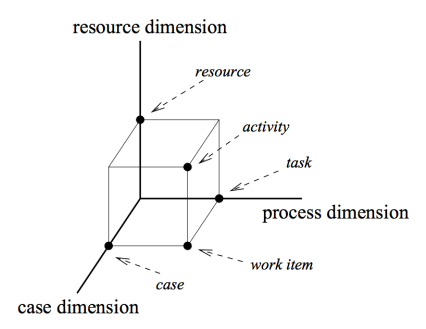
\includegraphics[width=8cm]{../figures/Workflow Dimensions.png}
    \caption{The three dimensions of workflows. (Image source:\cite{Malinao2017})}
    \label{WorkflowDimensions} 
\end{figure}
\indent Workflow models represent complex and dynamic real-world systems in various fields such as human resource management,  biology (integrated disease surveillance [Lopez et al. 2020]),  and manufacturing engineering (chiller systems \cite{Ramirez2024}). This includes models such as Petri nets (PN) and Robustness Diagrams with Loop and Time Controls (RDLT) \cite{Malinao2017}. These models allow workflow components to be analyzed and model properties to be verified. \\

\indent The study of the workflow model Robustness Diagrams with Loop and Time Controls has been important in recent years due to its capability to represent a workflow in all of its dimensions (process, resource, and case). Although there are other workflow models that can represent all dimensions e.g. business process modeling and notation (BPMN), activity diagrams, etc., there are gaps and challenges in verifying the properties of these models. Issues like concept excess, lack of support for explicit representation of data and rules, functional decomposition, etc. The dynamicity of RDLT allows it to be mapped to different mathematical models which enables different ways for the verification of model properties, such as soundness. \cite{Malinao2017} \\

\indent Classical soundness, in particular, refers to the property of a workflow to be absent of livelocks, deadlocks, and other anomalies in the flow \cite{Ramirez2024}. In general, to be classically sound, a model should have proper termination and liveliness. There are other notions of soundness derived from being classically sound, namely, relaxed, weak, easy, and lazy soundness. Relaxed soundness \cite{MalinaoPJS2023} is already defined as well as the easy, weak, and lazy notions of soundness \cite{Ramirez2024}, all of which differ in the degree of relaxations of proper termination and liveness \cite{MalinaoPJS2023}.\\  

\indent Hence, with all the knowledge about workflows and RDLT's notions of soundness, further research would expand in terms of automation to verify model properties. Therefore, various research has been done about the representation of RDLT into mathematical models aiming to automize verification. In Karen and Roben's work \cite{KarenRoben2018}, they proposed a matrix representation of RDLT to verify soundness. Asoy \cite{MalinaoPJS2023} used a matrix representation of RDLT to verify and automate classical soundness. This paper aims to leverage the structural behaviors of easy and weak soundness as formally defined by Ramirez (2024) and use matrix representations to verify these notions of soundness in an RDLT.


\section{Basic Definitions and Notations}
% -------------------------------------------
\subsection*{Robustness Diagram with Loop and Time Controls (RDLT)}
In this section, RDLT and its notions of soundness is defined. 
\indent RLDT is a workflow model that allows all three dimension of a workflow to be represented.

\begin{defn}\textbf{RDLT} \cite{Malinao2017}\\
    \label{RDLTDef}
    An RDLT is a graph representation \begin{math}R\end{math} of a system that is defined as \begin{math}R = (V, E, T, M)\end{math} where:
    \begin{itemize}
        \item \begin{math}V\end{math} is a finite set of vertices, where each vertex has a type \begin{math}V_{type}: V \rightarrow \end{math} \{'b', 'e', 'c'\} where 'b', 'e', and 'c' means the vertex is either a "boundary object", an "entity object", or a "controller", respectively.
        
        \item A finite set of arcs \begin{math}E \subseteq (V \times V) \backslash  E'\end{math} where \begin{math}E' = \{(x,y) | x,y \in V, V_{type}(x) \in \end{math} \{'b', 'e'\}, \begin{math}V_{type}(y) \in \end{math} \{'b', 'e'\}\} with the following attributes with user-defined values,
            
            \begin{itemize}
                \item \begin{math}C : E \rightarrow \Sigma \cup \{\epsilon\} \end{math} where $\Sigma$ is a finite non-empty set of symbols and $\epsilon$ is the empty string. Note that for real-world systems, a task \begin{math}v \in V\end{math}, i.e. \begin{math}V_{type}(v) = \end{math}'c', is executed by a component \begin{math}u \in V, V_{type}(u) \in \end{math} \{'b','e'\}. This component-task association is represented by the arc \begin{math}(u, v) \in E \end{math} where \begin{math}C((u,v)) = \epsilon\end{math}. Furthermore, \begin{math}C((x,y)) \in \Sigma\end{math} represents a constraint to be satisfied to reach \begin{math}y\end{math} from \begin{math}x\end{math}. This constraint can represent either an input requirement or a parameter \begin{math}C((x,y))\end{math} which needs to be satisfied to proceed from using the component/task \begin{math}x\end{math} to \begin{math}y\end{math}. \begin{math}C((x,y)) = \epsilon\end{math} represents a constraint-free process flow to reach \begin{math}y\end{math} from \begin{math}x\end{math} or a self-loop when \begin{math}x = y\end{math}.
                
                \item \begin{math}L : E \rightarrow \mathbb{Z}\end{math} is the maximum number of traversals allowed on the arc.
            \end{itemize}
        
        \item Let \begin{math}T\end{math} be a mapping such that \begin{math}T((x, y)) = (t1,...,tn)\end{math} for every \begin{math}(x, y) \in E\end{math} where \begin{math}n = L((x, y))\end{math} and \begin{math} t_{i} \in \mathbb{N}\end{math} is the time a check or traversal is done on \begin{math}(x, y)\end{math} by some algorithm’s walk on \begin{math}R\end{math}.
            
        \item \begin{math}M : V \rightarrow \{0,1\}\end{math} indicates whether \begin{math}u \in V\end{math} and every \begin{math}v \in V\end{math} where \begin{math}(u,v) \in E\end{math} and \begin{math}C((u,v)) = \epsilon\end{math} induce a sub-graph \begin{math}G_{u}\end{math} of \begin{math}R\end{math} known as a \textbf{reset-bound subsystem} (RBS). The RBS \begin{math}G_{u}\end{math} is induced with the said vertices when \begin{math}M(u) = 1\end{math}. In this case, \begin{math}u\end{math} is referred to as the \textbf{center} of the RBS \begin{math}G_{u}\end{math}. \begin{math}G_{u}\end{math}'s vertex set \begin{math}V_{G_{u}}\end{math} contains \begin{math}u\end{math} and every such \begin{math}v\end{math}, and its arc set \begin{math}E_{G_{u}}\end{math} has \begin{math}(x,y) \in E\end{math} if \begin{math}x,y \in V_{G_{u}}\end{math}.\\
        
        Finally, \begin{math}(a,b) \in E\end{math} is called an \textbf{in-bridge} of \begin{math}b\end{math} if \begin{math}a \notin V_{G_{u}}, b \in V_{G_{u}}\end{math}. Meanwhile, \begin{math}(b,a) \in E\end{math} is called an \textbf{out-bridge} of \begin{math}b\end{math} if \begin{math}b \in V_{G_{u}}\end{math} and \begin{math}a \notin V_{G_{u}}\end{math}. Arcs \begin{math}(a,b), (c,d) \in E\end{math} are \textbf{type-alike} if \begin{math}\exists y \in V\end{math} where \begin{math}(a,b), (c,d) \in Bridges(y)\end{math} with \begin{math}Bridges(y) = \{(r,s) \in E|(r,s)\end{math} is either an in-bridge or out-bridge of \begin{math}y\}\end{math} or if \begin{math}\forall y \in V, (a,b), (c,d) \notin Bridges(y)\end{math}.
    \end{itemize} 
\end{defn}

Figure \ref{sampleRDLT} shows an RLDT with a reset-bound system with center $x_2$ and its owned controllers $x_3$ and $x_4$. The in-bridges of the RBS with respect to $x_2$ are $(x_1, x_2)$ and $(x_6,x_2)$. Both arcs are type-alike with respect to $x_2$ as defined in \ref{RDLTDef}. However, $(x_3,x_2)$, being inside the RBS, is not type-alike to any of the aforementioned arcs. $(x_4, x_5)$ and $(x_4, x_6)$ are type-alike with respect to $x_4$.
For each arcs of this RDLT, $C-$ and $L-$ attributes are defined. The $x_1$ serves as the source, while the $x_7$ serves as the sink. 
\begin{figure} [H]
    \centering
    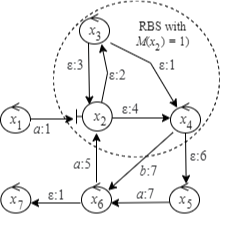
\includegraphics[width=6cm]{../figures/sampleRDLT.png}
    \caption{A Reset-Bound Subsystem-Containing Robustness Diagram with Loop and Time Controls with center at $x_2$, where $M(x_2)=1$. (Image source: \cite{MalinaoWCTP2023})}
    \label{sampleRDLT}
 \end{figure}
% Example RDLT (First Example)
% Figure \ref{RDLTComponents} shows an example of an RDLT based on the given definitions of the elements and the attributes that are labeled respectively. This RDLT also contains an RBS with the entity object $x2$ as the center of such RBS which is determined by its $M$-Attribute being equal to 1.\\
% \begin{figure}[H]
%     \centering
%     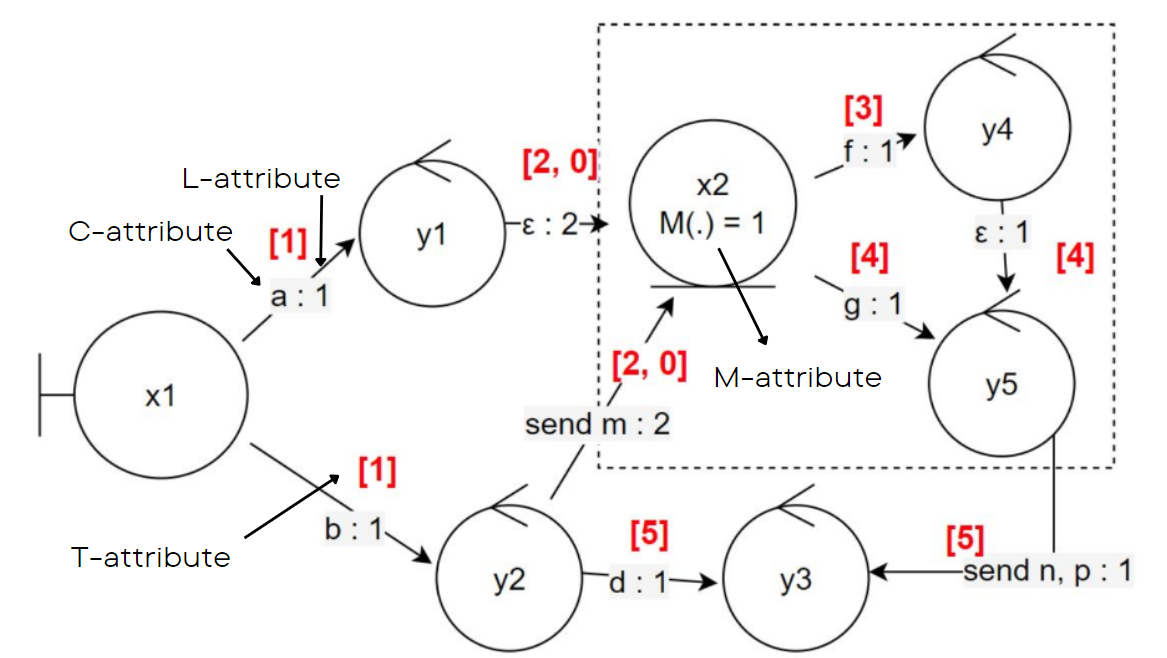
\includegraphics[width=12cm]{../figures/RDLT Components.png}
%     \caption{A Labeled Reset-Bound Subsystem-Containing Robustness Diagram with Loop and Time Controls with a Boundary Object $x1$, an Entity Object $x2$, and Controllers $y1$, $y2$, $y3$, $y4$, and $y5$. (Image source: \cite{Sulla2023})}
%     \label{RDLTComponents}
% \end{figure}

% -------------------------------------------
\subsection*{Activity Extraction Algorithm}
The proposed Activity Extraction algorithm in \cite{Malinao2017} takes an input RDLT \emph{R} with a defined start index \emph{s} and goal vertex \emph{f}. As shown in Algorithm \ref{ActivityExtraction} it returns an activity profile defined in \ref{activityProfile}, a set of exected vertices from the extracted activities.
To understand activity extraction fully, along with the definition of activity profile, reachability configuration, defined in \ref{reachabilityConfiguration}, is also first introduced.
\begin{defn}\label{reachabilityConfiguration}
    \textit{\textbf{Reachability Configuration}}\\
    A reachability configuration $S(t)$ in $R = (V, E, \Sigma, C, L, M)$ contains the arcs traversed by ${\mathcal A}$ at time step $t \in {\mathbb{N}}$.
\end{defn}
\begin{defn}\label{activityProfile}
    \textit{\textbf{Activity Profile}}\\
    A set $S = \{S(1), S(2), \ldots,$ $S(d)\}$ of reachability configurations, $d \in {\mathbb{N}}$, is an activity profile in $R = (V, E, \Sigma, C, L, M)$ where $\exists(u,v) \in S(1)$ and $(x,y) \in S(d)$ such that $\nexists w, z \in V$ where $(w,u), (y, z) \in E$. 
\end{defn}
Another definition, that of \emph{Unconstrained Arc} in \ref{unconstrainedarc} defines what an unconstrained arc is which allows for the traversal of arcs in activity extraction.

\begin{algorithm}[H]
    \caption{Activity Extraction Algorithm ${\mathcal A}$ \cite{Malinao2017, Sulla2023}}
    \label{ActivityExtraction}
    \begin{algorithmic}
        \State \textbf{Input:} $ R $, $ s \in V $, $ f \in V $
        \State \textbf{Output:} vertices $ S $ of $ R $, $ \emptyset $ otherwise
    \end{algorithmic}
    \begin{algorithmic}[1]
        \State Initialize $ S $
        \For{every $ (x,y) $}
            \State Initialize $ T((x,y)) $ such that $ T((x,y)) $ $ = $ $ (t_1, ..., t_n) $ where $ n $ $ = $ $ L((x,y)) $ and $ t_i $ $ \epsilon $ $ \mathbb{N} $ is the time a check or traversal is done on $ (x,y) $ by $ A $.
        \EndFor
        \State Let $ x $ $ = $ $ s $.
        \While{$ x $ $ \neq $ $ f $}
            \State Select $ (x,y) $ $ \epsilon $ $ E $ where $ L((x,y)) $ has not been reached.
            \If{$ \exists (u,x) $ $ \epsilon $ $ E $ $ = $ $ max(T((u,x))) $}
                \State Assign $ maxV $ $ + $ $ 1 $ to the leftmost zero of $ T((x,y)) $. 
            \Else
                \State $ maxV $ $ = $ $ 0 $.
            \EndIf
            \State Determine whether $ (x,y) $ is an unconstrained arc or not.
            \If{$ (x,y) $ is unconstrained}
                \State Traverse $ (x,y) $ .
                \State Assign $ MAX $ $ + $ $ 1 $ to $ T((x,y)) $ where $ MAX $ is the maximum value from all $ T((v',y)) $ $ \forall $ $ v' $ $ \epsilon $ $ V $ where $ (v',y),(v,y) $, and $ (x,y) $ are type-alike.
                \For{every $ (v,y) $ $ \epsilon $ $ E $ that is type-alike with $ (x,y) $}
                    \State Assign $ MAX $ $ + $ $ 1 $ to every $ T((x,y)) $.
                    \If{$ C((v,y)) $ $ \epsilon $ $ \Sigma $}
                        \State The last value in $ T((x,y)) $ where the last check was done on $ (v,y) $ is updated.
                    \ElsIf{$ v $ is either type 'b' or 'e' and $ y $ is type 'c'}
                        \State The first value in $ T((x,y)) $ is updated.
                    \EndIf
                \EndFor
            \ElsIf{$ (x,y) $ is not unconstrained and not other $ (x,y') $ $ \epsilon $ $ E $ where $ y' $ $ \epsilon $ $ V $ can be selected }
                \State Backtrack to $ a $ $ \epsilon $ $ V $ where $ (a,x) $ $ \epsilon $ $ E $ and $ a $ was previously visited by the algorithm to reach $ x $.
            \EndIf
        \EndWhile
        \If{activity extraction fails}
            \State \Return $ \emptyset; $
        \Else
            \State \Return $ S $
        \EndIf
    \end{algorithmic}
\end{algorithm}
\newpage
In step 4.3 of algorithm ${\mathcal{A}}$, an evaluation is performed to determine if $(x,y) \epsilon E$ is an unconstrained arc. The definition of an unconstrained arc is defined as follows:
\begin{defn} \label{unconstrainedarc}
    \textit{\textbf{Unconstrained Arc}}\\
    An arc $(x, y) \in E$ is \textbf{unconstrained} if $\forall (v,y) \in E$, where $(x,y)$ and $(v,y)$ are type-alike, any of the following traversal conditions hold, 
    \begin{enumerate}
        \item $C((v,y)) \in \{\epsilon, C((x,y))\}$,
        \item { $|\{t_i \in T((x,y))|t_i \geq 1\}| \leq  |\{t_j \in T((v,y))|t_j \geq 1\}|$ $\leq L((v,y)),$}
        \item $C((v,y)) \in \Sigma, C((x,y)) = \epsilon \wedge T(v,y) \neq [0]$.
    \end{enumerate}
    Note that $(x,y)$ will remain unconstrained (if it is such) regardless of any other $(v,y)$ where $(x,y)$ and $(v,y)$ are not type-alike.
\end{defn}
% -------------------------------------------
\subsection*{Vertex Simplification}
\begin{defn}\textbf{Vertex Simplified $R$} \cite{Malinao2017}\\
    \label{VertexSimpDef}
     A vertex-simplified RDLT $ G $ = ($ V' $, $ E' $, $ C' $) of $ R = (V, E, T, M) $ (with arc attributes $ C $ and $ L $) is a multigraph whose vertices $ v \in $ V have $ V_{type}(v) = 'c' $ where $ G $ is derived from $ R $ such that the following holds:
     \begin{enumerate}
         \item $ x \in V' $ if any of the following holds:
         \begin{itemize}
             \item $ x \in V $ and $ x \notin V_{G_u} $ of an RBS $ G_u $ in $ R $, or
             \item there exists an in-bridge $ (q, x) \in E $ of $ x \in V \cap V_{G_u}, q \in V $ of $ R $, or
             \item there exists an out-bridge $ (x, q) \in E $ of $ x \in V \cap V_{G_u}, q \in V $ of $ R $, or
         \end{itemize}
         \item $ (x, y) \in E' $ with $ C'((x, y)) = C((x, y)) $ for $ x, y \in V' $ if $ (x, y) \in E $
         \item $ C((x, y)) = \varepsilon $ if $ x, y \in V' \cap V_{G_u} $ and $ x $ is an ancestor of $ y $ in $ R $ and $ (x, y) \notin E_{G_u} $  
     \end{enumerate}

     We refer to this simplification of $ R $ as \textbf{level-1 vertex simplification} of $ R $ with respect to every RBS $ G_u $ in $ R $. A \textbf{level-2 vertex simplification} of $ R $ with respect to its RBS $ G_u $ is the level-1 vertex-simplification of $ G_u $ where $ G_u $ is treated as an RDLT where the value of the vertex attribute $ M $ of $ u $ is redefined to $ 0 $, i.e. $ M(u) $ $ = $ $ 0 $. With this, the verification of model properties (i.e. maximally composed and sound RDLTs) are separately done for the level-1 and level-2 vertex simplifications of $ R $. However, this separation does not affect the validity of proving for any of these properties on the entire RDLT itself. Furthermore, 
 \end{defn}

 In simpler terms, the vertices in \emph{R} present in a vertex-simplified RDLT \emph{G} are those that do not belong in any RBS or those inside an RBS but has an \emph{in-bridge} and/or an \emph{out-bridge}.
 The vertex-simplifications $R_1$ and $R_2$ of the RDLT in \ref{sampleRDLT} is shown in \ref{vertexSimplification}, respectively. $R_1$ captures a subgraph of $R$ found outside of its RBS, including the vertices of the RBS that have at least 1 in-brigde or out-bridge. $R_2$ vertex-simplification, however, captures the RBS itself. The vertices that have in- or out-bridges in $R$ are marked either as sources and/or sinks in $R_2$.
 \begin{figure}[H]
    \centering
    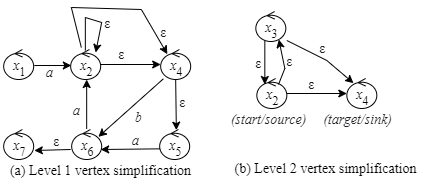
\includegraphics[]{../figures/vertexSimplification.png}
    \caption{The levels 1 and 2 vertex simplification $R_1$ and $R_2$ of the RLDT in \ref{sampleRDLT} (Image Source: \cite{MalinaoWCTP2023})}
    \label{vertexSimplification}
\end{figure}
% -------------------------------------------
\subsection*{L-Safeness of RDLTs}
% include here the defintions from kuya Ronnie's
% add paragraph introducing L-safeness of RDLT
In the analysis of processes in RDLT, particularly on its verification of soundness property, it is crucial that possible $L$-attrbute-based deadlocks are avoided. Reachability of the vertices relies heavily on the configuration of the arcs' $L-$values. The following definitions discusses the $L-$safeness with RDLTs from \cite{MalinaoPJS2023}.
\begin{defn}\textbf{Critical and Escape Arcs} \cite{MalinaoPJS2023}
    A cycle $ c $ $ = $ $ [ x_1 x_2 \ldots x_n ] $ is a sequence of vertices $ x_i $ $ \in $ $ V $, where $ (x_i,x_{i+1}) $ $ \in $ $ E $, $ i $ $ = $ $ 1,2, \ldots, n - 1 $, and no two vertices in $ c $ are the same except for $ x_1 $ $ = $ $ x_n $. The elements of $ c $ are denoted as $ Lit(c) $. We denote the set of arcs of $ c $ as $ ArcsOfCycle(c) $ $ = $ $ \{ (x,y) $ $ \in $ $ E | \exists x_i, x_{i+1} $ $ \in $ $ Lit(c) $ where $ x $ $ =  $ $ x_i $ and $ y $ $ = $ $ x_{i+1} \} $.

    $ (x,y) $ $ \in $ $ ArcsOfCycle(c) $ is called a critical arc (CA) in $ c $ if it has the minimum $ L $-value among the arcs in $ c $, i.e. $ L(x,y) $ $ = $ $ min_{(u,v) \in ArcsOfCycle(c) } \{L(u,v)\} $. If $ \exists (x,v) $ $ \in $ $ E $ such that $ v $ $ \in $ $ V \backslash Lit(c) $, then we refer to $ (x,v) $ as an escape arc (EA) of $ (x,y) $ in $ c $. Self-loops, i.e. $ (x,x) $, are cycles that are themselves entirely composed of one critical arc that does not affect the (re)use of other arcs in an RDLT.
\end{defn}

\begin{defn}\textbf{Loop-Safe Arcs} \cite{MalinaoPJS2023}
    \label{LSA}
    Let $ R $ be a connected RDLT, i.e. for every vertex $ v $ $ \in $ $ V $, there is a path from a source vertex $ s $ $ \in $ $ V $ to $ v $ in $ R $. A non-critical arc (NCA) $ (x,y) $ $ \in $ $ E $ of $ R $ is loop-safe if $ L(x,y) $ $ > $ $ RU(x,y) $, where
    \begin{gather*}
        RU(x,y) = \Sigma_{k=1^{|Cycles(x,y)|}} (I * L(u,v)) \text{, for some } (u,v) \in minL\_CA(c_k) \text{, with} \\
        I =
        \begin{cases}
            1, & \text{if } k = 1 \text{ or } \cup_{j=1^{k-1}} minL\_CA(c_j) \cap minL\_CA(c_k) \\
            0, & \text{otherwise,}
        \end{cases}
    \end{gather*}
    and $ minL\_CA(c) $ $ \subset $ $ E $ is the set of arcs whose $ L $-value is the minimum among the critical arcs found in $ c $, accounting the other cycles in $ c' $ in $ R $ that intersect with $ c $.
\end{defn}

\begin{defn}\textbf{Safe Critical Arcs} \cite{MalinaoPJS2023}
    \label{SafeCA}
    A CA $ (x,y) $ $\ in $ $ E $ is safe if there is an escape, non-critical arc $ (x,z) $ $\ in $ $ E $, where $ (x,z) $ is loop-safe.
\end{defn}
\subsubsection*{JOINs in RDLTs}
In RDLTs, it is not impossible for multiple processes to converge at a single vertex (JOIN). The type of join specifies how the incoming processes interact before proceeding in the workflow. The following definitions are the different types of joins in RDLTs:
\begin{itemize}
    \item[1.] AND-JOIN at $y \in V$: For every type-alike arcs $(v,y), (u,y) \in E$ where $(v,y) \neq (u,y)$, their C-values $C(v,y) \neq C(u,y)$ and $C(v,y),C(u,y) \in \Sigma$.
    \item[2.] MIX-JOIN at $y \in V$: There is at least one pair of type-alike arcs $(v,y), (u,y) \in E$ where $(v,y) \neq (u,y)$, $C(v,y) \neq C(u,y)$ and $C(v,y) = \epsilon$, and $C(u,y) \in \Sigma$.
    \item[3.] OR-JOIN: For every type-alike arcs $(v,y), (u,y) \in E$ where $C(v,y)=C(u,y)$.
\end{itemize}
The concept of JOIN-safe L-values ensures processes are in proper coordination with each other. This, along with \ref{LSA} and \ref{SafeCA}, provides the structural requirement for a classically sound RDLT, e.g, proper termination and liveness. These definitions serves as the basis for determining looser notions of soundness.
\begin{defn}\textbf{JOIN-safe L-values} \cite{MalinaoPJS2023}
    \label{JSL}
    For every pair of arcs $(u, y)$, $(v, y)$ $ \in $ $ E $, where $C(u, y)$ $ \neq $ $C(v, y)$, we say that $(u, y)$ and $(v, y)$ have JOIN-safe $L$-values if:

    \begin{enumerate}
        \item \textbf{One split origin.} There is exactly one common ancestor $ x $ $ \in $ $ V $ for $ u $ and $ v $ such that there is exactly one path $ P_u $ $ = $ $ a_1 a_2 \ldots a_n $, where $ a_1 $ $ = $ $ x $, $ a_{n-1} $ $ = $ $ u $, $ a_n $ $ = $ $ y $, $ a_i $ $ \in $ $ V $, $ 1 < I < n - 2 $, and another path $ P_v $ $ = $ $ b_1 b_2 \ldots b_m $, where $ b_1 $ $ = $ $ x $, $ b_{m-1} $ $ = $ $ v $, $ b_m $ $ = $ $ y $, $ b_j $ $ \in $ $ V $, $ 1 < j < m - 2 $. Furthermore, $ P_u $ and $ P_v $ do not intersect with each other except at $ x $ and $ y $. That is, no $ a_i $ and $ b_j $ along these paths are equal, for $ 1 < i < n $ $ 1 < j < m $; and
        \item \textbf{No unrelated process.} For every arc $ (a,b) $ $ \in $ $ E $, if $ a $ $ = $ $ x $, where $x$ is the one common ancestor of $u$ and $v$, then there is no path from $a$ to another vertex $r$ $\in$ $V$ such that for some $(r,s)$ $\in$ $ E $, $s$ $\neq$ $y$.
        \item \textbf{No branching out from every related process.} $\forall q_k $ $ \in $ $ Lit(P_q) $, where $ q $ $ \in $ $ \{u,v\} $, $ 1 \leq k < |Lit(P_q)| $, $ \nexists (q_{k,s}) $ $ \in $ $ E $ where $ s $ $ \in $ $ V \backslash Lit(P_q) $.
        \item \textbf{No process interruptions.} $ \forall q_k $ $ \in $ $ Lit(P_q) $, where $ q $ $ \in $ $ \{u,v\} $, $ 1 < k \leq |Lit(P_q)| $, $ \nexists (s,q_{k}) $ $ \in $ $ E $ where $ s $ $ \in $ $ V \backslash Lit(P_q) $.
        \item \textbf{Duplicate conditions.}
        \begin{itemize}
            \item If $ C(u,y) $, $ C(v,y) $ $ \in $ $ \Sigma $, i.e. an AND-JOIN at $ y $, then there is no process $ P $ $ = $ $ [x_1 x_2 \ldots x_p] $ in $ R $, where $ x_1 $ $ = $ $ x $, $ x_p $ $ = $ $ y $, such that $ C(x_{p-1}, x_p ) $ $ = $ $ C(u,y) $ (or $ C(v,y) $).
            \item Without any loss of generality, if $ C(u,y) $ $ = $ $ \varepsilon $ and $ C(v,y) $ $ \in $ $ \Sigma $, then any process $ P $ $ = $ $ x_1 x_2 \ldots x_p $ in $ R $, where $ x_1 $ $ = $ $ x $, $ x_p $ $ = $ $ y $, can have $ C(x_{p-1}, x_p) $ $ \in $ $ \{\varepsilon, C(v,y)\}$. That is, a MIX-JOIN can have duplicate conditions for the arcs connecting to $y$, but no two of such arcs have different conditions.
        \end{itemize}
        \item \textbf{Equal $ L $-values of arcs at the AND-JOIN.}
        \item \textbf{Loop-safe components of every related process.} For an AND- or MIX-JOIN merging at $y$, each of its processes $ P $ $ = $ $ x_1 x_2 \ldots x_k $, $ k $ $ \in $ $ \mathbb{N} $, where $ x_1 $ $ = $ $ x $ and $ x_k $ $ = $ $ y $, the arc $ (x_1, x_{i+1}) $ $ \in $ $ E $. $ i $ $ = $ $ 1, 2, \ldots, k - 1 $, is loop-safe. Lastly, for an OR-JOIN merging at $ y $, each process $ P $ $ = $ $ x_1 x_2 \ldots x_k $, $ k $ $ \in $ $ \mathbb{N} $, of this JOIN has its arc $ (x_i,x_{i+1}) $ to have a JOIN-safe L-value, $ i $ $ = $ $ 1, 2, \ldots, k - 1 $, if $ (x_i, x_{i+1}) $ is either a loop-safe arc or a safe CA in R.
    \end{enumerate}
    
\end{defn}
% -------------------------------------------
\subsection*{Reusability and Resets in RDLTs}
The concept of reusability refers to how components of an RDLT can be used in different situations, such as when an RDLT has an RBS \cite{MalinaoWCTP2023}. The information in this section is sourced from \cite{MalinaoWCTP2023} unless explicitly mentioned otherwise.

\begin{defn} Pseudocritical Arcs, Pseudo-escape Arcs \\
A pseudocritical arc $(PCA) (x,y) \in E$, where $(x,y)$ is a component of a cycle $c$ in $R$ where $L(x,y$) is the minimum among all the L-values of the arcs in $c$ which are not arcs of an RBS in $R$.

Meanwhile, a pseudo-escape arc $(PEA) (x,z) \in E$ is a non-critical arc in $R$ where $(x,y)$ and $(x,z)$ are type-alike.    
\end{defn}

\begin{defn} Expanded Reusability in RDLTs with Resets \\
Let $R =  (V, E, T, M)$ be a connected $RDLT$. If $\exists v \in V$ where $M(v)=1$, then let $B =  (V', E', T', M')$ be the RBS with its center $v$.
\begin{enumerate}
    \item Let $IB_r(X)$ be the set of in-bridges of $x \in V$.
    \item Let $Cycles_{part}(R)$ be a set of cycles in $R$ with the following property: $\forall p = [x_1 x_2 ... x_n] \in Cycles_{part}(R)$, there exist cycle components meeting these conditions:
    \begin{itemize}
        \item [(a)] $(x_i,x_{i+1}) \in E$ is inside an RBS $B$ of $R$ (i.e, $x_i,x_{i+1} \in V'$).
        \item [(b)] $(x_j,x_{j+1}) \in E$ is not inside $B$ (i.e, $x_j or x_{j+1} is not in V'$).
    \end{itemize}
\end{enumerate}
Whenever we have cycles $d = [d_1 d_2 ... d_{m1}], e = [e_1 e_2 ... e_{m1}] \in Cycles_{part}(R)$ that overlap in their non-RBS components, and this overlap contains both of their PCAs $(d_k,d_{k+1}), (e_{k'},e_{k'+1})$, where $L(d_k,d_{k+1}) \geq L(e_{k'},e_{k'+1})$, then consider only one of these PCAs. Choose the one with the minimum L-value as it would ultimately contribute to the reusability of every RBS component reachable from these cycle components.
\end{defn}

\begin{defn} (RU-preserving transformation) \\
    A transformation $\delta$ of an input RDLT $R$ to another RDLT $R'$ is said to be RU-preserving if for every activity profile $S = {S(1), S(2), ..., S(n_1)}, n_1 \in IN$, that is derivable from $R$, there is a corresponding activity profile $S' = {S'(1), S'(2), ..., S'(n_2)}, n_2 \in IN$, that is derivable from $R'$, where for every pair $(x,y) \in S(i)$ and $(y,z) \in S(i+1)$, either of the following holds:
    \begin{enumerate}
        \item $(x,y) \in S'(j)$ and $(y,z) \in S'(j+1)$,
        \item there exists a path $p=x_1, x_2, ..., x_n \in R$ being represented by the arc $(x_1, x_n)$ in $R$ being represented by the arc $(x_1, x_n)$ in $R'$ where $x_{k-1}=x,x_k, x_{k+1}=z$, and
            \begin{itemize}
                \item[(a)] $(s,x_1) \in S'(j)$ and $(x_1,x_n) \in S'(j+1)$, for some vertex $s$ in $R'$,
                \item[(b)] $(x_1,x_n) \in S'(j)$, for some $1 \leq j \leq n_2$, or
                \item[(c)] $(x_1,x_n) \in S'(j)$ and $x_n$, $s \in S_{j-1}$, for some vertex $s$ in $R'$.
            \end{itemize}
    \end{enumerate}
    Furthermore, we call $(x_1,x_n)$ as the abstract arc in $R'$ representing the path $p$ in $R$.
\end{defn}
% -------------------------------------------
\subsection*{Expanded Vertex Simplification}
The process of vertex simplification results to an RDLT lacking of $L$-values, both in $R_1$ and $R_2$. Therefore, \cite{MalinaoWCTP2023} proposes and extension of the process to produce \emph{expanded vertex simplifiction} $R_1'$ and $R_2'$ of $R$ by using the RDLT and its simplified vertex to retrieve the other attributes, e.g. $L$. The algorithm for producing $R_1'$ and $R_2'$ is outlined in \ref{EVSA}.
\begin{algorithm}
    \label{EVSA}
    \underline{\textbf{Expanded Vertex Simplification Algorithm(EVSA):}}\\
    \textbf{Inputs:} Let $R = (V, E, T, M)$ be an connected RDLT with an RBS, i.e. $\exists v \in V$, where $M(v) = 1$. Let $R_1 = (V_1, E_1)$ and $R_2 = (V_2, E_2)$ be the vertex simplifications of $R$. (The $C$-attributes of the arcs of $R$, $R_1$, and $R_2$ are denoted as $C$, $C_1$, $C_2$, respectively, while their $L$-attributes are $L$, $L_1$, and $L_2$, respectively.) \\

    \noindent
    \textbf{Outputs:} \textbf{Level 1 and Level 2 expanded vertex simplification} $R'_1 = (V'_1, E'_1, T'_1)$ and $R'_2 = (V'_2, E'_2, T'_2)$ of $R$, respectively . (The $C$-attributes of the arcs of $R'_1$ and $R'_2$ are $C'_1$ and $C'_2$, respectively, while their $L$-attributes are $L'_1$ and $L'_2$, respectively.)

    \begin{enumerate}
        \item For each $v \in V_1(V_2)$(or $V$ of $R$), set $v' \in V'_1(V'_2)$ to be its corresponding vertex, and if $(u,v) \in E_1(E_2)$, then its there is a corresponding arc $(u',v') \in E'_1(E'_2)$, where the $C$-values $C'_1(u',v')(C_2(u',v'))$ of $R'_1(R'_2)$ is set to $C(u,v)$ of $R_1(R_2)$, otherwise, none.  \\

        This step copies the vertices and arcs, inclusive of the $C$-values of $R_1$ and $R_2$ to their corresponding expanded versions $R'_1$ and $R'_2$, respectively. 

        \item For each $(u,v) \in E$, where $(u,v)$ is not in an RBS of $R$, and its corresponding arc $(u',v') \in V'_1$ of $L_1$, let $L'_1(u',v') = L(u,v)$. \\

        This step copies the $L$-values of $R$ for each of its arcs to the $L$-values of $R'_1$ whenever such arc does not belong to an RBS of $R$. 
        
        \item For each abstract arc $(u',v') \in E'_1$ of $R_1$, where $(u',v')$ represents the path \mbox{$p = x_1 x_2 \ldots x_n$} in $R$, i.e. $x_1 \in V$ and $x_n \in V$ correspond to $u' \in E'_1$ and  $v' \in E'_1$, respectively, set $L'_1(u',v') = \min\limits_{i = 1, \ldots, n-1} \{eRU(x_i, x_{i+1})\} + 1$. \\
        
        This step sets the $L$-value  of each abstract arc $(u',v')$ of $R'_1$ to reflect the maximum number of reuse of the path that it represents in $R$. Note that we treat each component of the RBS as an NCA relative to the non-RBS components, $eRU(u',v')$ must be greater than its reusability, e.g. greater than the PCAs of the cycles $(u',v')$ are involved in, hence, we add 1 to this maximum number of reuse. Additionally, note the $eRU$ of the arcs along the path $p$ can vary because of the reuse of such components within the RBS, albeit the number of times they are accessible through the in-bridges of their ancestor node is the same. However, the reusability of the entire path $p$ itself is bound to the minimum of the $L$-values of the arcs therein. Thus, this minimum shall be the representative $L$-value for these arcs as reflected by their representative abstract arc.
    \end{enumerate}
\end{algorithm}

\begin{figure}[H]
    \centering
    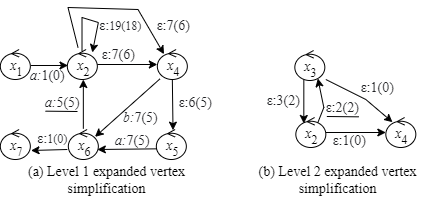
\includegraphics{../figures/expandedVertexSimplification.png}
    \caption{$R_1'$ and $R_2'$ expanded vertex simplification of the vertex simplified graphs in figure \ref{vertexSimplification}}
    \label{expandedVertexSimplifiedRLDTs}
\end{figure}
In simpler terms, the creation of a contraction path of a given vertex simplified RDLT $ G_1 $ or $ G_2 $, which can also be represented as $R_1$ and $R_2$ respectively, is the merging of a pair of vertices $ x $ and $ y $ connected by the arc $ (x,y) $ from the initial vertex through the contraction of arcs. Such a merging is only possible if the set of C-values of all arcs from $ x $ to $ y $ is a superset of the C-values of all arcs from other vertices in the subgraph towards $ y $ \cite{MalinaoWCTP2023}. This continues until the subgraphs $ R_1 $ and $ R_2 $ are represented as one vertex, if possible. This method is also referred to as the graph contraction strategy.

% -------------------------------------------
\subsection*{Soundness Property in RDLT}
On the soundness of RDLT, there are two formalized definitions of soundness, namely Classical and Relaxed Soundness \cite{Malinao2017,MalinaoPJS2023}. However, a recent formalization was also made for weak and easy soundness \cite{Ramirez2024}, the definitions of which are stated below.
\begin{defn}\textbf{Classical Soundness of RDLTs} \cite{MalinaoPJS2023}
    \label{ClassicalRDLTDef}
    An RDLT is of classical sound if and only if the following requirement is satisfied by each activity profile $ S = \{S(1), S(2), ..., S(k)\}, 1 \leq k \leq diam(R), diam(R) $ is the diameter of $ R $, of a set of source vertices $ I $ $ \subset $ $ V $ and a final output vertex $ f $ $ \in $ $ V, $ where $ \forall $ $ x $ $ \in $ $ I $ and $ y $ $ \in $ $ V $, $ (x,y) $ $ \in $ $ S(1), $ and $ (u,f) $ $ \in $ $ S(k) $, $ u $ $ \in $ $ V $:
    \begin{enumerate}
        \item \textbf{Proper termination.} For every activity profile $ S = \{S(1), S(2), ..., S(k)\}, 1 \leq k \leq diam(R) $, of a set of source vertices $ I $ $ \subset $ $ V $ and a final output vertex $ f $ $ \in $ $ V $.
        \begin{itemize}
            \item All arcs in the final reachability configuration $ S(k) $ must be incident to sink $ f $, i.e. for every $ (x,y) $ $ \in $ $ S(k), $ $ y = f $
            \item If $ k $ $ \leq $ $ 2 $: every arc incident to a vertex $ y $ in a reachability configuration $ S[i] $ has a corresponding arc incident from vertex $ y $ in a succeeding reachability configuration $ S(j) $, $ i.e. $ for every $ (x,y) $ $ \in $ $ S[i] $, there exists another arc $ (y,z) $ $ \in $ $ S(j) $, for all $ 1 \leq i < k $, and for some $ j $ in the range $ i + 1 \leq j \leq k $.
        \end{itemize}
        \item \textbf{Liveness.} Every arc is traversed in some activity profile, $ i.e. $ for every $ (x,y) $ $ \in $ $ E $, there is an activity profile $ S' = \{S'(1), S'(2), ..., S'(k')\} $, where $ (x,y) $ $ \in $ $ S'[i], 1 \leq k \leq k' $.
    \end{enumerate}
\end{defn}

Based on this definition, the first condition requires an RDLT \emph{R}'s each specified vertex and their subsequent vertices leading to the final vertex of \emph{R}. In other words, an RDLT needs to have proper termination. 
The second condition requires it to have no possible occurences of deadlocks for every component in the RDLT as it requires that all arcs are to be traversed to be included in the activity profile during extraction. Figure \ref{sampleRDLT} satisfies both conditions an is therefore classically sound.

\begin{defn}\textbf{Relaxed Soundness of RDLTs} \cite{Malinao2017, MalinaoPJS2023, Sulla2023}
    \label{RelaxedRDLTDef}
    An RDLT is of relaxed sound if for every sink $ f $ $ \in $ $ V $ and a source $ w $ $ \in $ $ R $, where $ w $ is an ancestor of $ f $, there exists an activity profile $ S = {S(1), S(2), ..., S(k)} $, where $ 1 \leq k \leq diam(R) $, where the following conditions hold:
    \begin{itemize}
        \item For every reachability configuration $ S(t) $ prior to $ S(k) $, if any, there should be at least one arc $ (x,y) $ $ \in $ $ S(t) $ and another arc $ (y,z) $ $ \in $ $ S(t') $, for a time $ t' $, where $ t < t' \leq k $. This ensures that there is at least one continuous path from $ w $ to $ f $ in activity $ S $.
        \item The final reachability configuration $ S(k) $ is only composed of arcs that point to the sink $ f $, $ i.e. $ $ \forall (x,y) $ $ \in $ $ S(k) $, $ y = f $.
        \item The set of arcs traversed at a time $ t $ is strictly contained in the set of arcs traversed at time $ t + 1 $, $ i.e. $ $ \bigcup_{i=1}^{t} S[i] $ $ \subset $ $ \bigcup_{i=1}^{t+1} S[i] $. Since an arc can occur in multiple $ S[i] $, the operator $ \bigcup $ should be considered a multiset union operator.
        \item Every arc $ (x,y) $ $ \in $ $ E $ is traversed in some activity profile $ S' $, $ i.e. $ there exists an activity profile $ S' $, where $ (x,y) $ $ \in $ $ S'(t) $ for some $ S'(t) $ $ \in $ $ S' $.
    \end{itemize}
\end{defn}
Relaxed soundness refers to a classically sound RDLT with the exception of the loosening of its proper termination. At least only one vertex is required to be leading to the final vertex, in contrast to a classically sound RDLT. This is given by the first, third, and fourth requirement. The liveness, however, is retained as defined in the second and third requirement, preventing deadlocks. Meaning, a relaxed soundness is live.  The RDLT therefore in figure \ref{sampleRDLT} is relaxed sound, aside from the fact that it is classically sound in the first place.

% -------------------------------------------


\section{Problem Statement}
Matrix representation is used to extract activities from an RDLT, using computations involving matrix operations. The purpose of this research is to verify the weak and easy soundness of an input RDLT using these operations. Karen and Roben \cite{KarenRoben2018} and Asoy \cite{Asoy2024} already conducted studies involving the matrix representation of relaxed and classical soundness, respectively. Similarly, the recently formalized notion of soundness, that of weak and easy soundness in RDLT \cite{Ramirez2024}, provided a behavioral and structural profile upon which algorithms were proposed for the verification thereof. The problem statement of this paper is to create a matrix representation for the verification of weak and easy soundness of RDLT, based on its formalizations.
% objectives of the study
\section{Aim of the Work}
\subsection*{General Objectives}
Currently, there are already existing literature on weak and easy soundness in the context of RDLT. However, in the case of this research, the matrix representation for the verification of these notions of soundness is to be addressed. Therefore, we shall address the following general objectives:
\begin{enumerate}
    \item To incorporate matrix operations on the matrix representation of RDLT to verify easy and weak soundness;
    \item To design a matrix representation of RDLT to verify easy and weak sound- ness; and
    \item To create an algorithm for the verification of RDLT using matrix repre- sentation.
\end{enumerate}
\subsection*{Specific Objectives}
In alignment with the general objectives, the following specific objectives are identified to reach these aims:
\subsubsection*{For Weak Soundness Structural Verification}
\begin{enumerate}
    \item To establish matrix representation and operations for the verification of deadlock tolerance in both level 1 and level 2 expanded vertex simplification graphs, $R_1$ and $R_2$, respectively, of RDLT $R$.
    \item To establish matrix representation and operations for the verification that $R$ is deadlock-resolving.
    \item To generate a list of deadlock points in $R$ and identify escape contraction paths.
    \item To establish matrix representation and operations for the verification of weakened-join safeness of $R$.
    \item To establish matrix representation and operations to verify weakened join-safe values of every split-join pair in $R$.
    \item To verify the loop-safeness of NCA and safeness of CA\@.
    \item To measure the time and space complexity of the matrix-based verification of weak soundness of $R$.
\end{enumerate}
\subsubsection*{For Easy Soundness Structural Verification}
\begin{enumerate}
    \item To establish matrix representation and operations for the verification of a contraction path existing from the source to the sink vertex.
    \item To measure the time and space complexity of the matrix-based verification of easy soundness of R.
\end{enumerate}
% scopes and limitations
\section{Scope and Limitations}
The scope and limitations of the study are the following:
\begin{enumerate}
    \item The study will focus on the design of matrix representation that encapsulates the structure of RDLT. It will incorporate matrix operations on the verification of the structural profiles of RDLT to determine its weak and easy soundness. The study will not delve to alternative models other than matrix representation.
    \item The study will center on RDLT as the main structural model to verify notions of soundness with. Furthermore, its level 1 and level 2 expanded vertex simplified graphs will be used in the verification of weak soundness. The study will not explore other types of models beyond these graphs.
    \item The study will center on the verification of weak and easy notions of soundness. Its structural profiles will be used for the verification. The study does not include other notions of soundness.
    \item The study will focus on verifying deadlock tolerance in the context of RDLT, as defined in the structural profile of weak soundness. The study is limited to the definition of deadlock tolerance within this context.
    \item The study aims to design and implement a matrix-based verification algorithms for weak and easy notions of soundness of an RDLT. The algorithms are only limited to weak and easy soundness and will not perform matrix operations beyond these verifications.
\end{enumerate}

% significance of the study
\section{Significance of the Study}
\indent The study and its results will contribute to the enhanced understanding of RDLT and the verification of notions of soundness. Specifically, the study is centered on the matrix-representation of RDLT to verify weak and easy soundness, which could lead to improved methods for the analysis and modeling of complex systems. This deepens the theoretical framework of RDLT and strengthens its applicability in systems design. By establishing matrix-representation and operations for the verification of these notions of soundness, we address gaps and contirbute to the broader understanding of the field by:
\begin{enumerate}
    \item Providing a structured framework for the verification of easy and weak soundness, which could lead to the enhancement of reliablity and accuracy of complex systems.
    \item Introduce efficient deadlock detection and resolution mechanisms through matrix-based operations, leading to more robust systems.
    \item Providing the groundwork for the advancement of automated verification tools, speeding up the validation process of RDLTs, in the scope of weak and easy notions of soundness.
\end{enumerate}

\section{Theoretical and Conceptual Framework}
The figure presents the conceptual framework of the research. It contains required concepts and definitions in order to proceed with the methodology and achieve the reseach objectives. 

The main requirements for acheiving the main objectives of the research are the following: definition of RDLT \cite{Malinao2017}, definition of a weak and easy sound RDLT based on their structural and behavioral profiles \cite{Ramirez2024}, RDLT Activity extraction \cite{Malinao2017} \cite{Asoy2024}, Vertex Simplification, and Matrix Operations \cite{KarenRoben2018}. RDLT is defined in [maam malinao] and the classical notion of soundness. By the scope of this research, the weak and easy notions of soundness are to be verified, the profiles and algorithm of which are already defined by \cite{Ramirez2024}. Majority of the research's objectives is focused on the matrix-based verification of the deadlock tolerance (and its subsequent properties) of the input RDLT. This methodology requires vertex simplification \cite{Malinao2017} (both level-1 and level-2) and a proposed algorithm for activity extraction \cite{Malinao2017}. Finally, the final state vector output of the matrix operations on the input RDLT will be evaluated for its validity, then its weak and easy soundness.

The implementation of this research would therefore include the reusing of the definitions of RDLT \cite{Malinao2017}, weak and easy soundness profiles \cite{Ramirez2024}, and the algorithm for the verification thereof. The algorithm by \cite{Ramirez2024} would be translated or modified to verify a matrix-based RDLT, represented by R's final state vector after activity extraction. To achieve these main objectives, specific objectives are to be achieved first, requiring the same set of concepts and algorithms. Finally, the calculation of time and space complexity of the matrix-based verification of weak and easy soundess will also be performed. 


\begin{figure}[p]
    \centering
    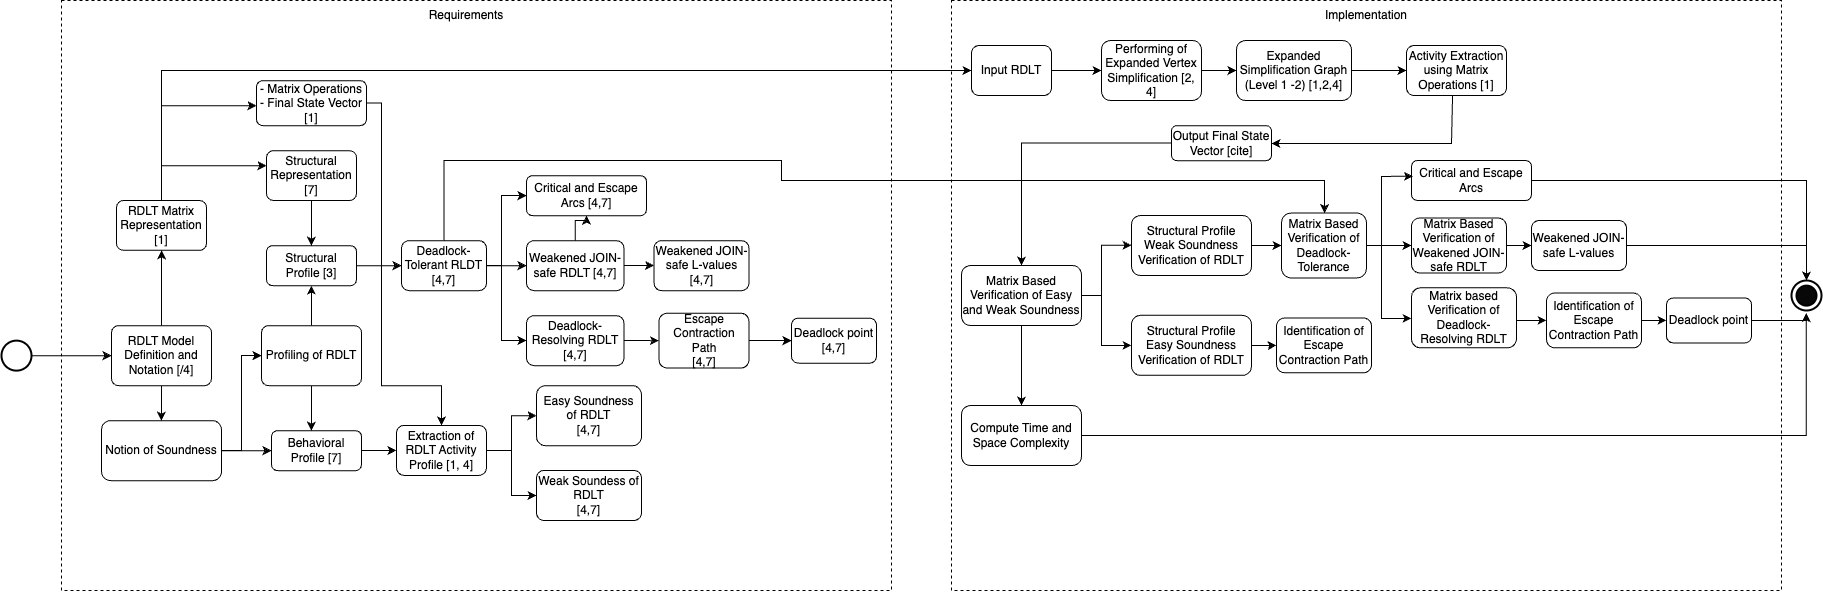
\includegraphics[width=\paperwidth, angle=90]{../figures/Conceptual Framework.png}
    \caption{This framework shows the requirements of the research's framework, with its main components, namely: Matrix Representation, Behavioral and Structural Profile of the RDLT}
\end{figure} %iintroduction
\chapter{Review of Related Literature}
\section*{On Weak and Easy Notions of Soundness in RDLTs}
Recent formalizations on the definition of weak and easy soundness of RDLT and their structural and behavioral profiles allow the basis for the verification of the said properties. The following definitions are from \cite{Ramirez2024} and contains the weak and easy notions of soundness, its behavioral and structural profiles, and the proposed algorithms for the verification (and the time and space complexity) thereof based on each notion's definitions.
The information under this section is taken from the fundamental work of \cite{Ramirez2024} unless explicitly stated otherwise.
% ---------------------------
% Weak Soundness Notion of RDLTs
\section{Weak Soundness Notion of RDLTs}

\begin{defn}[\textbf{Weak Soundness of RDLTs}] 
    \label{WeakRDLTDef}
    An RDLT $ R $ is of weak soundness if and only if the following requirement is satisfied by each activity profile $ S = \{S(1), S(2), ..., S(k)\}, 1 \leq k \leq diam(R), diam(R) $ is the diameter of $ R $, of a set of source vertices $ I $ $ \subset $ $ V $ and a final output vertex $ f $ $ \in $ $ V, $ where $ \forall $ $ x $ $ \in $ $ I $ and $ y $ $ \in $ $ V $, $ (x,y) $ $ \in $ $ S(1), $ and $ (u,f) $ $ \in $ $ S(k) $, $ u $ $ \in $ $ V $:
    \begin{enumerate}
        \item \textbf{Proper termination.} For every activity profile $ S = \{S(1), S(2), ..., S(k)\}, 1 \leq k \leq diam(R) $, of a set of source vertices $ I $ $ \subset $ $ V $ and a final output vertex $ f $ $ \in $ $ V $.
        \begin{itemize}
            \item All arcs in the final reachability configuration $ S(k) $ must be incident to sink $ f $, i.e. for every $ (x,y) $ $ \in $ $ S(k), $ $ y = f $
            \item If $ k $ $ \leq $ $ 2 $: every arc incident to a vertex $ y $ in a reachability configuration $ S(i) $ has a corresponding arc incident from vertex $ y $ in a succeeding reachability configuration $ S(j) $, i.e. for every $ (x,y) $ $ \in $ $ S(i) $, there exists another arc $ (y,z) $ $ \in $ $ S(j) $, for all $ 1 \leq i < k $, and for some $ j $ in the range $ i + 1 \leq j \leq k $.
        \end{itemize}
    \end{enumerate}
\end{defn}
Based on this definition, an RDLT is of weak soundness if it properly terminates, where every reached vertex in each activity profile of the RDLT leads to the sink. In the context of WF-Nets, this notion of soundness in RDLT is similar in a sense that it does not require the workflow to be live. A weak sound RDLT allows for arcs to not be traversed at all. \\
In figure \ref{RDLTWeak}, a weak sound RDLT is shown. All the arcs leading to $x_5$ from $x_4$ can be traversed, except with the path starting from the arc $(x_1, x_2)$, since it cannot be traversed.
\begin{figure}[H]
    \centering
    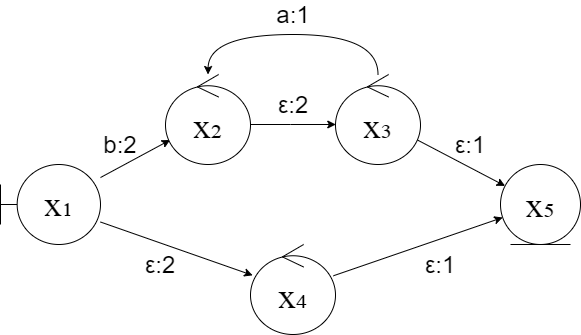
\includegraphics[width=12cm]{../figures/RDLT Weak.png}
    \caption{An RDLT of Weak Soundness (Image Source: \cite{Ramirez2024})}
    \label{RDLTWeak}
\end{figure}

% ---------------------------
% Easy Soundness Notion of RDLTs
\section{Easy Soundness Notion of RDLTs}

\begin{defn}\textbf{Self-Controlling Arc}
    \label{SelfCA}
    A self-controlling arc is a profile of an RDLT $ R $ where a MIX-JOIN or AND-JOIN at vertex $ x $ can never be resolved. 
\end{defn}

Figure \ref{SelfControllingArc}, shown below, is an example of a self-controlling arc as defined in Definition \ref{SelfCA}. In this case, vertex $ b $ is the vertex that can never resolved due to one of the components of the AND-JOIN that violates the unconstrainedness criterion of the activity extraction algorithm.

\begin{figure}[H]
    \centering
    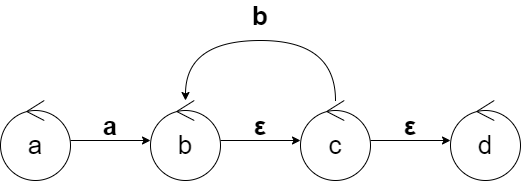
\includegraphics[width=12cm]{../figures/Self-Controlling Loop.png}
    \caption{An RDLT of Easy Soundness Image Source: \cite{Ramirez2024}}
    \label{SelfControllingArc}
\end{figure}

\begin{defn}\textbf{Easy Soundness of RDLTs}
    \label{EasyRDLTDef}
    An RDLT $ R $ is of easy soundness if and only if the following requirement is satisfied by an existing activity profile $ S = \{S(1), S(2), ..., S(k)\}, 1 \leq k \leq diam(R), diam(R) $ is the diameter of $ R $, of a set of source vertices $ I $ $ \subset $ $ V $ and a final output vertex $ f $ $ \in $ $ V, $ where $ \forall $ $ x $ $ \in $ $ I $ and $ y $ $ \in $ $ V $, $ (x,y) $ $ \in $ $ S(1), $ and $ (u,f) $ $ \in $ $ S(k) $, $ u $ $ \in $ $ V $:
    \begin{enumerate}
        \item \textbf{Option to complete.} There exists an activity profile $ S = \{S(1), S(2), ..., S(k)\}, 1 \leq k \leq diam(R) $, of a set of source vertices $ I $ $ \subset $ $ V $ and a final output vertex $ f $ $ \in $ $ V $ where there exists a path $ P $ composed of $ P = x_1, x_2 \cdots x_n $ with $ i = 1, 2 \cdots n - 2 $ where $ (x_i, x_{i+1}) $ $ \in $ $ S(i), (x_{i+1}, x_{i+2}) $ $ \in $ $ S(j), i < j, x_i = s $ and $ x_n = f $.
    \end{enumerate}
\end{defn}

As described in this definition, the only requirement for any given RDLT to be easy sound its sink to be reachable from the source. It does not require proper termination that all reached vertices must have a path that eventually leads to the sink, unlike weak soundness \ref{WeakRDLTDef}. Figure \ref{RDLTEasynotLazy} shows an easy sound RDLT. A deadlock exist due to $x_2$ since there is no path from this vertex that will reach the sink $x_6$. However, there still exist a path from $x_1$ to the sink $x_6$ through the arcs $(x_1,x_5)$, $(x_5,x_6)$, fulfilling the requiremnts for an easy sound RDLT.

\begin{figure}[H]
    \centering
    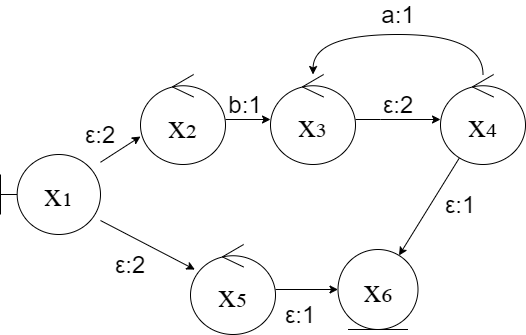
\includegraphics[width=12cm]{../figures/RDLT Easy.png}
    \caption{An RDLT of Easy Soundness Image Source: \cite{Ramirez2024}}
    \label{RDLTEasy}
\end{figure}

\begin{rem}
    Within the context of WF-Nets, the difference between lazy and easy soundness is the number of completed cases where each case instance is represented by a token. Specifically, lazy soundness requires that there should be only one token that reaches the sink place while easy soundness allows multiple tokens in the sink place.
    
    Currently, the activity extraction algorithm for RDLTs, as described in \cite{Malinao2017}, is within the sequential context and therefore only represents one continuous case. With this, it is concluded that, sequentially, the definition of lazy and easy soundness are the same. However, lazy and easy soundness of RDLTs can be differentiated with the use of parallel activity extraction as multiple parallel cases can be visualized through this \cite{Doñoz2024}. This difference is shown in Figure \ref{RDLTEasynotLazy} with the sequential and parallel activity profiles. For the parallel activity, a traversal tree is utilized to visualize the various activities that are happening simultaneously. This visualization aims to structurally show and identify the parallel and non-parallel activities through observing the termination time for each branch as proposed in \cite{Doñoz2024}.

    \begin{figure}[H]
        \centering
        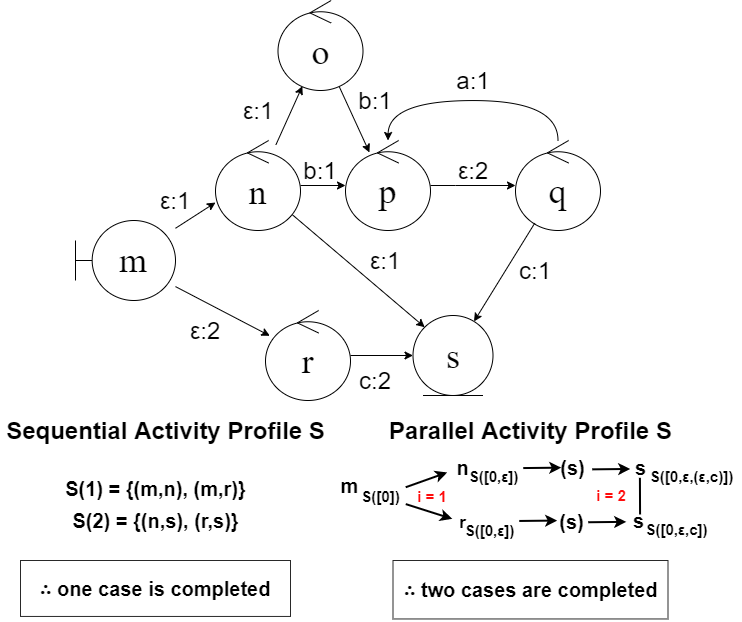
\includegraphics[width=16cm]{../figures/RDLT Parallelized Easy not Lazy w Exp.png}
        \caption{An Parallelized RDLT of Easy but not Lazy Soundness (Image Source: \cite{Ramirez2024})}
        \label{RDLTEasynotLazy}
    \end{figure}
\end{rem}
% ---------------------------
% Behavioral Profiles of Weak and Easy Soundness of RDLTs
\section{Behavioral Profiles of Weak and Easy Sound RDLTs}

This section introduces theorems that define the behavioral profiles of both weak-sound and easy-sound RDLTs.

\begin{thm}[Implication of Weak Soundness from Classical Soundness of an RDLT $ R $] 
    \label{CtWRDLT}
    If an RDLT $ R $ is of classical sound, then it is of weak sound.
\end{thm}

\begin{proof}
    Let $ R $ be a classical sound RDLT.

    Assume that $ R $ is not of weak sound. With this, then the following claim must hold:

    \begin{enumerate}
        \item There exists an activity profile $ S = \{S(1), S(2), ..., S(k)\}, (q,o) $ $ \in $ $ S(k), q $ $ \in $ $ V, k $ $ \in $ $ \mathbb{N}, $ in $ R, $ where $ \exists (p, u) $ $ \in $ $ S(i), 1 \leq i < k, $ such that $ \nexists(u,y) $ $ \in $ $ \bigcup_{j=i+1}^{k} S(j) $. This means that $ S $ does not properly terminate through $ (p,u) $ $ \in $ $ S(i) $, i.e. the child $ y $ $ \in $ $ V $ of $ u $ is a pending task of an unfinished process in $ S $.
    \end{enumerate}
    % For this claim, $ (p,u) $ can either have the following cases:

    % \begin{enumerate}
    %     \item $ (p,u) $ leads to an AND-join merging at $ y $ $ \in $ $ V $, where $ \exists(v,y) $ $ \in $ $ E $, where $ C(u,y) $ 
    %     $ \in $ $ \Sigma, C(u,y) $ $ \neq $ $ C(v,y) $, and an unchecked $ C(v,y) $ results in an unresolved AND-join at y. Through this, both $ (u,y) $ and $ (v,y) $ were never traversed by the algorithm such that there exists a reachability configuration $ S(j) $ where $ (u,y), (v,y) $ $ \in $ $ S(j) $ and $ i < j \leq k $.
    %     \item $ (p,u) $ leads to a MIX-join merging at $ y $ $ \in $ $ V $, where $ C(u,y) $ $ = $ $ \varepsilon $, and $ \exists(v,y) $ $ \in $ $ E $, where $ C(v,y) $ $ \in $ $ \Sigma $, such that an unchecked $ C(v,y) $ leads to the conclusion that both arcs are unconstrained, thus including them in $ S $.
    %     \item $ (p,u) $ leads to an OR-join where a path $ P $ leads to an output $ o' $ $ \in $ $ V $, where $ o' $ $ \neq $ $ o $ which is in turn the sink vertex of $ R $. Through this, $ \exists(a,b) $ $ \in $ $ S(n) $ of the activity profile where $ b $ $ \in $ $ V \ \{o\} $.
    % \end{enumerate}

    As proved in Theorem 1 of \cite{MalinaoPJS2023}, an RDLT $ R $ has been proved to terminate properly given that $ R $ is classical-sound. Through this, a classical sound RDLT satisfies the sole requirement of proper termination that an RDLT of weak soundness must have.
\end{proof}
% ---------------------------
% Structural Profiles of Weak and Easy Soundness of RDLTs
% ---------------------------
\begin{thm}[Implication of Easy Soundness from Weak Soundness of an RDLT $ R $] 
    If an RDLT $ R $ is of weak sound, then it is of easy sound.
    \label{WtERDLT}
\end{thm}

\begin{proof}

    Let R be a weak sound RDLT and assume it is not of easy sound. Through this, it is assumed that there is no activity profile that has a path from the source that eventually leads to the sink.
    
    As proven in Theorem \ref{PTWeak}, the given weak-sound self-controlling RDLT was found to have proper termination even without liveness. With this, it was also proven that it had the option to complete as there must exist a path from $ x $ to the sink vertex. Through this, a weak-sound RDLT satisfies the sole requirement of the option to complete that an RDLT of easy soundness must have.
    
\end{proof}

\begin{cor}[Implication of Easy Soundness from Classical Soundness of an RDLT R]
    If an RDLT $ R $ is classical sound, then it is of easy sound.
    \label{CtERDLT}
\end{cor}

\begin{proof}
    Follows from Theorem \ref{CtWRDLT} and \ref{WtERDLT}.
\end{proof}

\section{Structural Profiles of Weak and Easy Sound RDLTs}

This section introduces theorems that define the structural profiles of both weak-sound and easy-sound RDLTs.

\begin{thm}[Proper Termination of an RDLT $ R $ of Weak Soundness] 
    A weak sound RDLT $ R $ properly terminates even without the requirement of liveness.
    \label{PTWeak}
\end{thm}

\begin{proof}

    Let $ R $ be a self-controlling RDLT where deadlocks occur at $(u,y)$. Let $ R $ also be an RDLT of weak soundness.
    
    Due to the existence of deadlocks, $ R $ is considered to be an RDLT that is not live. To prove that a $ R $ still exhibits proper termination, we need to first establish that $ R $ is able to complete through reaching the sink vertex from the source vertex.
    
    In this case, the activity extraction algorithm reaches $ x $ at $S(t)$ through $v$, i.e $(v, x)$ $ \in $  $ S(t)$. If there exists $(u, y) $ $ \in $ $ E $ and $ C(u, y) $ $ \in $ $ \Sigma $, then $ (u,y) $ is constrained. Since $ R $ is of weak soundness, then there must exist a path $ P = x_1, x_2, ... x-{n-2} $ where $ x_1 = x $ and $ x_{n-2} $ $ = $ $ f $, the sink vertex.
    
    As we now have proven the completion of R, we move on to proving its proper termination by assuming that there exists a path $ P $ $ = $ $ x ... f $ and $ P’$ $ = $ $ x ... f $ where $ P $ $ \neq $ $ P’ $ i.e both arrive at the same sink vertex but they overlap with each other. If the components of $ P $ and $ P’ $ are in $ S $, then they form a MIX-join or an AND-join. Moreover, since paths $ P $ and $ P’ $ both complete in $ S $, then both paths complete at the same time which proves proper termination.
    
\end{proof}

As discussed in Chapter 1, \cite{MalinaoPJS2023} verifies the classical soundness of an RDLT if it satisfies the requirements of JOIN-safe $L-$values and $L-$safeness. \cite{Ramirez2024} propsed an algorithm that takes a similar approach that uses the initial requirements and weakening them, allowing the lack of liveness in a given RDLT.
\begin{defn}\textbf{Weakened JOIN-safe $ L $-values}
    \label{WJVals}
    For every split-join pair of arcs $ (u,y) $, $ (v,y) $ $ \in $ $ E $ in an RDLT $ R $, $ (u,y) $ and $ (v,y) $ have weakened JOIN-safe $ L $-values if the following conditions are met:
    \begin{itemize}
        \item For every process with $ C(u,y) $ or $  C(v,y) $ $ = $ $ \varepsilon $
        \begin{enumerate}
            \item CAs are allowed as long as they are safe, i.e there exists a loop-safe non-critical EA for each CA.
            \item Branching out is allowed as resolving its JOIN is not affected by the arc that has a $ C $-value of $ \varepsilon $.
            \item Process interruptions are allowed regardless of the $ C $-values of the interrupting arc.
        \end{enumerate}
        \item For every process with $ C(u,y) $ or $  C(v,y) $ $ = $ $ \Sigma $
        \begin{enumerate}
            \item \textbf{One-split origin for sibling processes merging at an AND- or MIX-JOIN.} There is one common ancestor $ x $ $ \in $ $ V $ for $ u $ and $ v $ such that there are is a pair of sibling processes $ P_u $ $ = $ $ a_1 \ldots a_n $, where $ a_i $ $ = $ $ x $, $ a_{n-1} $ $ = $ $ u $, $ a_n $ $ = $ $ y $, $ a_i $ $ \in $ $ V $, $ 1 < I < n - 2 $, and $ P_v $ $ = $ $ b_1 \ldots b_m $, where $ b_j $ $ = $ $ x $, $ b_{m-1} $ $ = $ $ v $, $ b_m $ $ = $ $ y $, $ b_j $ $ \in $ $ V $, $ 1 < I < m - 2 $.  Since both paths are siblings, then they must have no arcs in common, i.e. they do not intersect except at $ x $ at $ y $; and
            \item \textbf{No unrelated processes.} For every arc $ (a,b) $ $ \in $ $ E $, if $ a $ $ = $ $ x $, where $ x $ is the one common ancestor of $ u $ and $ v $, then there is no path from $ a $ to another vertex $ r $ $ \in $ $ V $ such that for some $ (r,w) $ $ \in $ $ E $, $ w $ $ \neq $ $ y $.
            \item \textbf{No branching out from every related process.} $ 
            \forall q_k $ $ \in $ $ Lit(P_q) $, where $ q $ $ \in $ $ \{u,v\} $, $ 1 \leq k < |Lit(P_q)| $, $ \nexists (q_{k,s}) $ $ \in $ $ E $ where $ s $ $ \in $ $ V \backslash Lit(P_q) $. This is to ensure that the JOIN is resolved.
            \item \textbf{Process interruptions.} With any loss of generality, if the interrupting arc $ (w,v) $ $ \in $ $ E $ has a $ C $-value of $ \varepsilon $, then process interruptions are allowed.
            \item \textbf{Duplicate values.} 
            \begin{itemize}
                \item If $ C(u,y) $, $ C(v,y) $ $ \in $ $ \Sigma $, i.e. an AND-JOIN at $ y $, then there is no process $ P $ $ = $ $ [x_1 x_2 \ldots x_p] $ in $ R $, where $ x_1 $ $ = $ $ x $, $ x_p $ $ = $ $ y $, such that $ C(x_{p-1}, x_p ) $ $ = $ $ C(u,y) $ (or $ C(v,y) $).
                \item Without any loss of generality, if $ C(u,y) $ $ = $ $ \varepsilon $ and $ C(v,y) $ $ \in $ $ \Sigma $, i.e. a MIX-JOIN at $ y $, then any process $ P $ $ = $ $ x_1 x_2 \ldots x_p $ in $ R $, where $ x_1 $ $ = $ $ x $, $ x_p $ $ = $ $ y $, can have $ C(x_{p-1},x_p) $ $ \in $ $ \{ \varepsilon, C(v,y) \} $, i.e. duplicate $ C $-values are allowed but no two of such arcs must have different $ C $-values.
            \end{itemize}
            \item \textbf{Equal $ L $-values of arcs at the AND-JOIN.}
            \item \textbf{No CAs exist within the process.} 
        \end{enumerate}
    \end{itemize}
\end{defn}

In comparison to the requirements of JOIN-safe L-values as described in Definition \ref{JSL}, the requirements for weakened JOIN-safe L-values is more lenient as the name suggests. Specifically, the fourth requirement is weakened such that it now allows process interruptions given that their $ C $-value is equal to $ \varepsilon $. Although it retains the first six requirements from the JOIN-safe L-values definition, it replaces the requirement of the loop-safeness of all related process with the requirement that there are no CAs within the process. Through these changes, this allows deadlocks to occur given that it does not occur within JOINs that has a process with a C-value with $ \Sigma $. 

\begin{defn}\textbf{Weakened JOIN-safe RDLT $ R $}
    \label{WJRDLT}
    An RDLT $ R $ is weakened JOIN-safe if every split-join pair in $ R $ has weakened JOIN-safe $ L $-values.
\end{defn}

\begin{defn}\textbf{Deadlock Point}
    \label{DLP}
    A deadlock point is each vertex $ x $ $ \in $ $ dV $ in an RDLT $ R $ where $ dV $ is a set of vertices in $ R $ and $ dV $ $ \subset $ $ V $, such that $ x $ $ \in $ $ dV $ is unreachable at some time step of the activity extraction algorithm.
\end{defn}

\begin{defn}\textbf{Escape Contraction Path}
    \label{ECPath}
    An escape contraction path is a path $ P = x_1, x_2 \ldots x_n $ in an RDLT $ R $ such that the following holds:
    \begin{enumerate}
        \item $ x_1 $ is a parent of a deadlock point in $ R $, i.e. $ x_1 $ $ = $ $ p $ where $ (p,q) $ $ \in $ $ E $ and $ q $ $ \in $ $ dV $, and
        \item $ P $ is a contraction path from $ x_1 $ to $ x_n $ in $ R $ where $ x_n $ is the sink vertex of $ R $.
    \end{enumerate}
\end{defn}

Definitions \ref{DLP} and \ref{ECPath} both describe the structures that must both exist simultaneously in a weak-sound RDLT as it assures that such an RDLT properly terminates even with the presence of deadlocks. As an example, vertex $ x_2 $ in Figure \ref{RDLTWeak} is the deadlock point of the RDLT as it is unreachable at the first time step of the activity. The escape contraction path in this case is $ P $ $ = $ $ x_1, x_4, x_5 $ where $ x_1 $ is the parent of the deadlock point $ x_2 $ and $ x_5 $ is the sink vertex.

\begin{defn}\textbf{Deadlock-Resolving RDLT $ R $}
    \label{DLResolving}
    An RDLT $ R $ is deadlock-resolving if for every deadlock point $ x \in V $, there exists at least one escape contraction path from a parent of $ x $ to the sink in R.
\end{defn}

\begin{lem}
    An expanded vertex simplification $ R_i $, where $ i $ $ = $ $ 1, 2 $, is deadlock-tolerant if and only if every activity thereof properly terminates.
\end{lem}

\begin{defn}\textbf{Deadlock-Tolerant RDLT $ R $}
    An RDLT $ R $ is deadlock-tolerant if every NCA is loop-safe, every CA is safe, $ R $ is weakened JOIN-safe and deadlock-resolving.
\end{defn}

With these definitions, the structural definition of a weak-sound RDLT is defined in Theorem \ref{SVWeak}.

\begin{thm}\textbf{Structural Verification of the Weak Soundness of an RDLT $ R $}
    \label{SVWeak}
    An RDLT $ R $ is weak-sound if and only if both the level-1 and level-2 expanded vertex simplifications of R, $ R_1 $ and $ R_2 $ respectively, are deadlock-tolerant.
\end{thm}

With Theorem \ref{SVWeak} as the basis, Algorithm \ref{WeakAlg} verifies the weak soundness of a given input RDLT $ R $ through the satisfaction of the requirements of deadlock-tolerance.

\begin{algorithm}[H]
    \caption{Weak RDLT Soundness Verification Algorithm (WRSVA) }
    \label{WeakAlg}
    \begin{algorithmic}
        \State \textbf{Input:} RDLT $ R $ with or without RBS
        \State \textbf{Output:} True, false otherwise
    \end{algorithmic}
    \begin{algorithmic}[1]
        \State Apply Expanded Vertex Simplification Algorithm \cite{MalinaoWCTP2023}
        \If{$ R $ contains an RBS}
            \State $ i $ $ = $ $ 2 $
        \Else
            \State $ i $ $ = $ $ 1 $
        \EndIf
        \For{every vertex simplification $ R_i $}
            \For{every vertex $ v $ $ \in $ $ V $}
                \State Store deadlock point $ y $
            \EndFor
            \For{every deadlock point $ y $ $ \in $ $ V $}
                \State Determine if a non-critical loop-safe escape contraction path exists from $ y $
                \State Determine if the split-join pair containing $ y $ has weakened JOIN-safe L-values
            \EndFor            
        \EndFor
        \If{$ R_1 $ is deadlock-tolerant}
            \If{$ R $ contains an RBS}
                \If{$ R_2 $ deadlock-tolerant}
                    \State \Return true
                \EndIf
            \EndIf
            \State \Return true
        \Else
            \State \Return false
        \EndIf
    \end{algorithmic}
\end{algorithm}

\begin{thm}\textbf{Time Complexity of WRSVA}
    The time complexity of verifying that an RDLT $ R $ is weak-sound is $ O(c|E|^4) $.
    \label{TCWRSVA}
\end{thm}
\begin{proof}
    The algorithm is divided into three main processes: (1) expanded vertex simplification \cite{MalinaoWCTP2023}, (2) determining the deadlock-points, and (3) verifying deadlock tolerance. For the first process, it has a time complexity of $ O(|V|^2)$ which corresponds to the maximum number of arcs $ R $ can have. Because the algorithm visits every arc of the diagram to replicate them or create abstract versions for the outputs $ R_1 $ and $ R_2 $ (if an RBS exists), the worst-case scenario for this algorithm is when the RDLT has the maximum amount of arcs, hence $ O(|V|^2) $. 
    
    For the second process, it has a time complexity of $ O(|V|+|E|)$, where it corresponds to the sum of the number of vertices $ V $ and arcs $ E $ in $ R $. This process uses the depth-first or breadth-first search algorithm to solve the problem, hence $ O(|V|+|E|) $.

    The third process of verifying deadlock tolerance can be divided into its four requirements which has their own processes: (1) verifying loop-safeness, which takes $ O(c|E|^4) $ time \cite{MalinaoPJS2023}, (2) verifying existence of safe critical arcs, which takes $ O(|E|^2) $ time \cite{MalinaoPJS2023}, (3) verifying weakened JOIN-safeness, and (4) verifying deadlock resolution.
    
    The verification of weakened JOIN-safeness can be further divided into its component processes and determining each of their time complexities. Specifically for every AND- and MIX-JOIN, it concerns the processes of (1) determining the one split origin, (2) determining if there are no unrelated process, (3) determining if there are no branches, (4) determining if there are no processes interruptions with a C-value of $ Sigma $, (5) determining duplicate conditions at the merge point, (6) determining the equality of the L-values, and (7) determining the non-existence of critical arcs. The first three processes take $ O(|V||E|^2) $ time \cite{MalinaoPJS2023}. The fourth process takes $ O(|V||E|) $ time, similar to its stricter counterpart in \cite{MalinaoPJS2023} where it avoids all process interruptions no matter the $ C $-attribute. The fifth and sixth processes takes $ O(|V||E|log|E|) $ and $ O(|V||E|) $ time respectively \cite{MalinaoPJS2023}. The last process to determine the number takes $ O(c|E|) $ where $ c $ is the number of cycles as it is the highest time complexity of the required steps to find so, specifically Problem 1 to 3 in Lemma 1 of \cite{Malinao2017}. Because the dominating processes in terms of time complexity are the first three processes, the time complexity of verifying weakened JOIN-safeness is $ O(|V||E|^2) $.

    Lastly, verifying if the RDLT $ R $ is deadlock-resolving requires $ O(p(|V| + |E|)) $ where $ p $ signifies the number of deadlock points since deadlock-resolving is essentially the process of graph contraction, which takes $ O(|V| + |E|) $ \cite{MalinaoPJS2023}, for every deadlock point in $ R $.
    
    With the time complexities of the sub-processes of deadlock tolerance, verifying loop-safeness has the greatest complexity out of the processes, making the time complexity of determining deadlock tolerance is $ O(c|E|^4) $.

    Since the time complexity of the determining deadlock tolerance is greater out of the processes as well, the weak soundness of $ R $ can be determined in $ O(c|E|^4) $ time.
\end{proof}

\begin{thm}\textbf{Space Complexity of WRSVA}
    The space complexity of verifying that an RDLT $ R $ is weak-sound is $ O(|E|^2) $.
    \label{SCWRSVA}
\end{thm}
\begin{proof}
    As mentioned earlier, the algorithm is divided into three main processes. For the first process of EVS, it has a space complexity of $ O(|V|^2)$ which corresponds to the maximum number of arcs $ R $ can have. Because the algorithm stores every arc of the diagram to replicate them or create abstract versions for the outputs $ R_1 $ and $ R_2 $ (if an RBS exists), the worst-case scenario for this algorithm is when the RDLT has the maximum amount of arcs, hence $ O(|V|^2) $. 
    
    For the second process, it has a space complexity of $ O(|V|+|E|)$ similar to its time complexity. It stores the vertices and arcs traversed to create the contraction path as it uses the depth-first or breadth-first search algorithm to solve the problem, hence $ O(|V|+|E|) $.

    The third process of verifying deadlock tolerance can be divided into its four requirements which has their own processes: (1) verifying loop-safeness, which takes $ O(c|E|) $ space \cite{MalinaoPJS2023}, (2) verifying existence of safe critical arcs, which takes $ O(|v|+|E|) $ space \cite{MalinaoPJS2023}, (3) verifying weakened JOIN-safeness, and (4) verifying deadlock resolution.
    
    The verification of weakened JOIN-safeness can be further divided into its component processes and determining each of their space complexities. Specifically for every AND- and MIX-JOIN, it concerns the processes of (1) determining the one split origin, (2) determining if there are no unrelated process, (3) determining if there are no branches, (4) determining if there are no processes interruptions with a C-value of $ Sigma $, (5) determining duplicate conditions at the merge point, (6) determining the equality of the L-values, and (7) determining the non-existence of critical arcs. The first five processes as well as the last process use $ O(|E|^2) $ space \cite{MalinaoPJS2023}. However, the sixth process uses $ O(|V||E|) $ space. Because the sixth process needs the least amount of space and is the sole process with a different complexity, the space complexity of verifying weakened JOIN-safeness is $ O(|E|^2) $.

    Lastly, verifying if the RDLT $ R $ is deadlock-resolving requires $ O(p(|V| + |E|)) $ space similar to its time needed as this process is similar to the graph contraction for every deadlock point in $ R $.
    
    With the space complexities of the sub-processes of deadlock tolerance, verifying loop-safeness has the greatest complexity out of the processes, making the time complexity of determining deadlock tolerance is $ O(|E|^2) $.

    Since the space complexity of the determining deadlock tolerance is greater out of the processes as well, the weak soundness of $ R $ can be determined with $ O(|E|^2) $ space.
\end{proof}

Shown below is Theorem \ref{SVEasy} that describes the structural requirements required to determine the easy soundness of an RDLT.

\begin{thm}\textbf{Structural Verification of the Easy Soundness of an RDLT $ R $}
    \label{SVEasy}
    An RDLT $ R $ is easy-sound if and only if the following elements exist: 
    \begin{itemize}
        \item A contraction path $ P_1 $ in the level-1 vertex simplification $ R_1 $ of $ R $ from the initial vertex $ x_i $ to the final vertex $ x_f $, wherein $ P_1 $ $ = $ $ x_1, \ldots, x_f $
        \item A contraction path $ P_2 $ in the level-2 vertex simplification $ R_2 $ of $ R $ from the initial vertex $ z $ to the final vertex $ p $ of the RBS, wherein $ P_2 $ $ = $ $ z, \ldots, p $
        \item An in-bridge $ (x,y) $ formed by a component in $ P_1 $ such that there exists a component $ (y,z) $ in $ P_2 $
        \item An out-bridge $ (q,p) $ formed by a component in $ P_2 $ such that there exists a component $ (p,r) $ in $ P_1 $
    \end{itemize}
\end{thm}

With Theorem \ref{SVEasy} as the basis, Algorithm \ref{EasyAlg} verifies the easy soundness of a given input RDLT $ R $ through the satisfaction of a contraction path existing from the source to the sink vertex.

\begin{algorithm}[H]
    \caption{Easy RDLT Soundness Verification Algorithm (ERSVA) }
    \label{EasyAlg}
    \begin{algorithmic}
        \State \textbf{Input:} RDLT $ R $ with or without RBS
        \State \textbf{Output:} True, false otherwise
    \end{algorithmic}
    \begin{algorithmic}[1]
        \State Apply Vertex Simplification Algorithm \cite{Malinao2017}
        \If{$ R $ contains an RBS}
            \State $ i $ $ = $ $ 2 $
        \Else
            \State $ i $ $ = $ $ 1 $
        \EndIf
        \For{every vertex simplification $ R_i $}
            \State Apply Graph Contraction Strategy \cite{Malinao2017}
        \EndFor
        \If{$ R_1 $ has a contraction path from the source $ x_1 $ to the sink $ x_n $}
            \If{$ R $ contains an RBS}
                \If{$ R_2 $ has a contraction path from the source $ z $ to the sink $ p $}
                    \State \Return true
                \EndIf
            \EndIf
            \State \Return true
        \Else
            \State \Return false
        \EndIf
    \end{algorithmic}
\end{algorithm}

To illustrate this verification of easy soundness, Figure \ref{VSEasy} depicts the step-by-step application of ERSVA to the easy sound RDLT shown in Figure \ref{RDLTEasy}. Since such an RDLT does not have an RBS, then it represents the level-1 vertex simplification and does not have a level-2 vertex simplification. Although this contraction does not result in one singular vertex representing all the vertices in the original figure, there exists a contraction path from the initial vertex $ x_1 $ to the final vertex $ x_6 $. This proves that the option to complete requirement is satisfied by the RDLT, thus verifying its easy soundness.

    \begin{figure}[H]
        \centering
        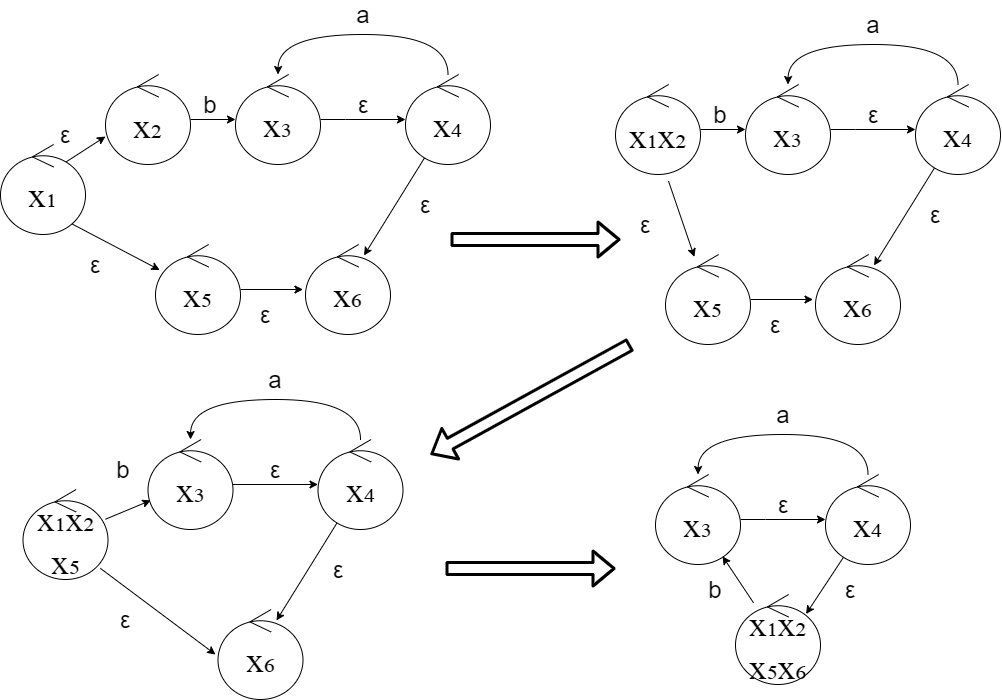
\includegraphics[width=15cm]{../figures/SV Easy Sound RDLT.png}
        \caption{An Parallelized RDLT of Easy but not Lazy Soundness}
        \label{VSEasy}
    \end{figure}

\begin{thm}\textbf{Time Complexity of ERSVA}
    The time complexity of verifying that an RDLT $ R $ is easy-sound is $ O(|V|^2) $.
    \label{TCERSVA}
\end{thm}
\begin{proof}
    The algorithm is divided into two main processes: (1) vertex simplification \cite{Malinao2017} and (2) graph contraction \cite{Malinao2017, MalinaoPJS2023}. For the first process, it has a time complexity of $ O(|V|^2)$ which corresponds to the maximum number of arcs $ R $ can have. Because the algorithm visits every arc of the diagram to replicate them or create abstract versions for the outputs $ R_1 $ and $ R_2 $ (if an RBS exists), the worst-case scenario for this algorithm is when the RDLT has the maximum amount of arcs, hence $ O(|V|^2) $. 
    
    For the second process, it has a time complexity of $ O(|V|+|E|)$, where it corresponds to the sum of the number of vertices $ V $ and arcs $ E $ in $ R $, because the process essentially determines if there exists a path from the source vertex to every vertex. Although this process is only done to make sure that there is a path from the source to the sink vertex, this complexity still applies as a worst-case scenario when there are no deadlocks within $ R $, i.e. $ R $ is live. As proved in \cite{MalinaoPJS2023}, this process uses the depth-first or breadth-first search algorithm to solve the problem, hence $ O(|V|+|E|) $.

    Since the time complexity of the vertex simplification is greater out of the two processes, the easy soundness of $ R $ can be determined in $ O(|V|^2) $ time.
\end{proof}

\begin{thm}\textbf{Space Complexity of ERSVA}
    \label{SCERSVA}
    The space complexity of verifying that an RDLT $ R $ is easy-sound is $ O(|V|^2) $.
\end{thm}
\begin{proof}
    Similar to the time complexity, the algorithm is divided into the vertex simplification and graph contraction. 
    
    For the first process, it has a space complexity of $ O(|V|^2)$ as the process stores every arc within $ R $ to generate $ R_1 $ and $ R_2 $ if $ R $ has an RBS. The worst-case scenario is $ R $ having the maximum amount of arcs given a number of vertices $ V $,  hence $ O(|V|^2) $. 

    For the second process, it has a space complexity of $ O(|V| + |E|) $ \cite{MalinaoPJS2023} as the process stores the vertices and arcs to simulate the possible contraction path of both the vertex simplifications. 

    Since the space complexity of the vertex simplification is greater out of the two processes, the easy soundness of $ R $ can be determined using $ O(|V|^2) $ space.
\end{proof}
\newpage
\section*{On the Matrix Representation of the Verification of Soundness}
\subsection*{} %RRL
\chapter{Methodology}

\begin{comment}
    Outline of the Methodology:
    - Introduction
    - Verification of Deadlock-Resolving RDLT
        - Contraction Path Generation (for identificaiton of deadlocks)
        - identification of escape contraction paths
        - Matrix-based algorithm for verification of Deadlock-Resolving RDLT
    - Loop-Safeness and Safeness Verification (Matrix-based)
    - Weakened JOIN-Safeness Verification (Matrix-based)
    - Weak Soundness of RDLT Verification (Matrix-based)
    - Easy Soundness of RDLT Verification (Matrix-based)

\end{comment}

This section introduces a matrix-based implementation of the verfication of weak and easy soundness of RDLT. The general algorithm for these verification is based on the formalizations of \cite{Ramirez2024} in terms of structural verifications of the said soundness properties. 

Firstly, on weak soundness, \cite{Ramirez2024} proposed WRSVA in which Deadlock-Tolerance is verified in order to verify weather or not an RDLT is weak sound. As explained in the related literatures, deadlock-tolerance refers to an RDLT being deadlock-resolving, having all NCAs loop-safe, CAs safe, and having all its split-join pairs as weakened JOIN-safe. All of these properties are verified through the use of matrices and their corresponding operations. The proofs and test-cases are also outlined for each verification of these mentioned properties. 

Similarly, easy soundness verification as formalized by \cite{Ramirez2024} is also implemented using matrix representation and operations. Its property of having an option to complete is verified by finding a contraction path from the source of R to the sink. Corresponding proofs and test-cases are also included to this proposed method. 

\subsection{Verification of Deadlock-Resolving RDLT}
% I think I should include a reference of the theorems from Ramirez' regarding his definitions. 
Theorem 3.4.3 in \cite{Ramirez2024} explains that an RDLT $R$ is of weak soundness if and only if both level-1 and level-2 vertex simplifications of $R$ are deadlock-tolerance. The paper defines deadlock-tolerance as an RDLT where every $NCA$ are loop-safe, every $CA$ are safe, $R$ is weakened JOIN-safe, and is deadlock-resolving.

For the verification of whether $R$ is deadlock-resolving, the matrix representation of which includes the enumeration of relevant deadlocks in $R$, and the identification of the existence of escape contraction paths from the parent of each deadlocks. The existence of an escape contraction paths is what ensures proper termination albeit the existence of deadlocks within an RDLT, removing the liveness property. Therefore, such RDLT is of weak soundness.

\subsubsection*{Identification of Deadlocks}
On the identification deadlocks, a method is proposed which involves the contraction \cite{Malinao2017} of the expanded vertex simplified RDLT $R_i$. This contraction algorithm as proposed by Malinao in here dissertation checks the c-verifiability of the RDLT \cite{Malinao2017}. Two adjacent vertices are contractable or can be merged when the arc currently being checked has contraint/s which is a subset of all the contraints coming towards the other vertex the algorithm is trying to contract. The final contraction shows the contraction path, which is a path of vertcies, that are reachable through an activity, hence through activity extraction, as well. That said, no unreachable vertices will be included in the contracted vertices, hence deadlocks, as defined in \cite{Ramirez2024}, can be identified.

This paper implements a matrix-based contraction algorithm adopted from the modified contraction algorithm (MCA) introduced in \cite{malinao2024model}. The following sections define the necessary matrices and algorithms to achieve a research objective. 

% Matrices 

\begin{defn} \textbf{Adjacency Matrix $RV_{adj}$} \\
Let $R_i = \bigl(V_i, E_i,\Sigma_i, C_i, L_i, M_i\bigr)$ be an expanded vertex simplification of an RDLT $R$. The $n \times n$ matrix of a directional graph, where $n = |V_i|$ and the rows and columns correspond to the vertex set $V_i = \{\,v_1, v_2, \ldots, v_n\}$ at time step $t$, is defined as

\[
  RV_{adj}^{t} \;=\;
  \begin{pmatrix}
    RV_{\mathrm{adj}}(v_1,v_1) & RV_{\mathrm{adj}}(v_1,v_2) & \cdots & RV_{\mathrm{adj}}(v_1,v_n) \\[6pt]
    RV_{\mathrm{adj}}(v_2,v_1) & RV_{\mathrm{adj}}(v_2,v_2) & \cdots & RV_{\mathrm{adj}}(v_2,v_n) \\[6pt]
    \vdots                    & \vdots                    & \ddots & \vdots                    \\[6pt]
    RV_{\mathrm{adj}}(v_n,v_1) & RV_{\mathrm{adj}}(v_n,v_2) & \cdots & RV_{\mathrm{adj}}(v_n,v_n)
  \end{pmatrix}.
\]

Each entry $RV_{adj}(x,y)$ represents the number of distinct arcs from $x$ to $y$, given by
\[
  RV_{adj}(x,y) \;=\;
  \begin{cases}
    RV_{adj}(x,y) \in \mathbb{N}, & \text{if } (x,y)\,\in E_i \text{ in } R_i, \\[5pt]
    0,     & \text{otherwise}.
  \end{cases}
\]
\end{defn}

\begin{defn} \textbf{Constraints Matrix $RV_C$} \\
We similarly define the matrix $RV_c$. The $n \times n$ matrix of a directional graph, where $n = |V_i|$ and the rows and columns correspond to the vertex set $V_i = \{\,v_1, v_2, \ldots, v_n\}$ at time step $t$, is defined as
\[
   RV_{C}^{t} \;=\;
  \begin{pmatrix}
    RV_c(v_1,v_1) & RV_c(v_1,v_2) & \cdots & RV_c(v_1,v_n) \\[6pt]
    RV_c(v_2,v_1) & RV_c(v_2,v_2) & \cdots & RV_c(v_2,v_n) \\[6pt]
    \vdots        & \vdots        & \ddots & \vdots        \\[6pt]
    RV_c(v_n,v_1) & RV_c(v_n,v_2) & \cdots & RV_c(v_n,v_n)
  \end{pmatrix}.
\]
Each entry $RV_{C}^{t}(x,y)$ represents the corresponding C-attribute of the arcs from $x$ to $y$ in the Adjacency Matrix, given by
\[
  RV_{C}^{t}(x,y) \;=\;
  \begin{cases}
    C(x,y)\in \Sigma \cup \{\epsilon\}, & \text{if } (x,y)\in E_i \text{ in } R_i,\\[5pt]
    \varnothing,                                  & \text{otherwise}.
  \end{cases}
\]
\end{defn}

\newpage
 
\begin{algorithm}[H]
\caption{\textbf{Matrix-based Contraction Path Generation}}
\label{alg:contractionPathGeneration}
\textbf{Given} RDLT R; Pre-processing Steps:

\textbf{Input}: Expanded vertex simplification $R_i$ of RDLT R

\textbf{Output}: Contraction Path P

\textbf{Matrices}: $RV^{t}_{\text{adj}}$ and $RV^{t}_{\text{C}}$

    \begin{algorithmic}[1]

    \State Initialize C-Attribute Matrix $RV^{0}_{\text{C}}$ of $R_i$
    \State Let $s' \in V_i$ be the source and $f' \in V_i$ be the sink
    \State Let $x = s'$
    \State Initialize $P = \{x\}$
    \State Let $t = 1$

    % \While{$P$ does not contain $f'$}
    % \While{\exists\, x \in X}
    % \While{\exists $y$ \in $V_i$}
    \While{$\exists y \in V_i \mid RV^{t-1}_{\text{adj}}(x,y) \geq 1$}

        \State $\mathcal{Y} \leftarrow \{ y \in V_i \mid RV^{t-1}_{\text{adj}}(x,y) \geq 1 \}$
        \State Select any $y \in \mathcal{Y}$
        \State Let $\text{LHS} = RV^{t-1}_{C}(x,y) \cup \{\epsilon\}$
        \State $\mathcal{U} \leftarrow \{ u \in V_i \mid u \neq x \wedge (RV^{t-1}_{\text{adj}}(u,y) \geq 1) \}$
        \State Let $\text{RHS} = \bigcup_{u \in \mathcal{U}} RV^{t-1}_{C}(u,y)$
        \If {$\text{LHS} \supseteq \text{RHS}$}
            \State Update $RV^{t-1}_{C}(u,y) = \epsilon, \forall (u,y) \in E_i, u \neq x$
            \ForAll {$u \in \mathcal{U}$}
                \State $RV^{t-1}_{C}(u,y) = \epsilon$
            \EndFor
            \State Let $z = x \land y$
            \State Let $z = xy$ = Matrix Addition of rows (columns) $x$ and $y$ in $RV^{t-1}_{\text{adj}}$
            \ForAll {$w \in V_i$}
                \State RowMerge\_Adj: $RV^{t}_{\text{adj}}(z,w) = RV^{t-1}_{\text{adj}}(x,w) + RV^{t-1}_{\text{adj}}(y,w)$
                \State ColMerge\_Adj: $RV^{t}_{\text{adj}}(w,z) = RV^{t-1}_{\text{adj}}(w,x) + RV^{t-1}_{\text{adj}}(w,y)$
            \EndFor
            \State Let $z = xy$ = Element-wise Set Union of rows (columns) $x$ and $y$ in $RV^{t-1}_{C}$
            \ForAll {$w \in V_i$}
                \State RowMerge\_C: $RV^{t}_{C}(z,w) = RV^{t-1}_{C}(x,w) \cup RV^{t-1}_{C}(y,w)$
                \State ColMerge\_C: $RV^{t}_{C}(w,z) = RV^{t-1}_{C}(w,x) \cup RV^{t-1}_{C}(w,y)$
            \EndFor
            \State $V_i = (V_i \setminus \{x,y\}) \cup \{z\}$
            \State Create $RV^{t}_{\text{adj}}$ as an $m \times m$ matrix where $m = n - t$ and as the submatrix of $RV^{t-1}_{\text{adj}}$ with rows and columns indexed by updated vertex set $V_i$ of $R_i$
            \State Create $RV^{t}_{C}$ as an $m \times m$ matrix where $m = n - t$ and as the submatrix of $RV^{t-1}_{C}$ with rows and columns indexed by updated vertex set $V_i$ of $R_i$
            \State Let $x = z$
            \State Let $P = P \cup \{y\}$
            \State Let $t = t + 1$
        \EndIf
    \EndWhile
    \State \textbf{return} P
    \end{algorithmic}
\end{algorithm}

Algorithm \ref{alg:contractionPathGeneration} performs the first phase of MCA in \cite{MalinaoJuayongScienggj2024} with some modification. Instead of doing the contraction until the sink, this algorithm \ref{alg:contractionPathGeneration} performs the contraction until there is no vertex that can be contracted, leaving the unreachable vertices as not part of the merged vertices. This process involves checking the constraints coming from vertex $x$ to $y$ and verifying whether those set of constraints is a superset of all the constraints of arcs coming towards $y$. If so, then $x$ and $y$ can be contracted. With this procedure, $Points of Delay$ ($POD$)\cite{Malinao2017} vertices will not be merged, at least if there is no looping arc towards those points which can resolve the constraints making them reachable at some time step $t$. $POD$s are vertices that cannot be visited immediately due to the unresolved constraints of its incoming arcs.


\subsubsection*{Verification of the Existence of Escape Conctraction Paths}
After the identification of deadlocks in $R$, in order to verify whether or not it is deadlock resolving as per its definition, each deadlock should have an escape contraction path \cite{Ramirez}. Additionally, the parents involved in this verification are only the reachable ones.

Then, the proposed algorithm will go through each parent of each deadlock to verify the existence of an escape contraction path. 


\begin{algorithm}[H]
\caption{\textbf{Matrix-Based Finding Escape Contraction Path Algorithm}}
\label{alg: findEscapeConractionPath}
\textbf{Given}: RDLT $R_i$; Preprocessing


\textbf{Input}: Parent Vertex $w$, Sink $f'$, Contraction Path $P$, Adjacency Matrix of $R_i$ $RV_{adj}$

\textbf{Output}: Boolean, $True$, otherwise $False$  

\begin{algorithmic}[1]
    \State Initialize $Visited[0...n-1] \gets false$ \Comment for each vertex in $V_i$
    \State Initialize $Q \gets$ empty queue
    \State $Q.queue(w)$
    \State $Visited[w] \gets true$
    \While{$Q \neq \emptyset$}
        \State $current \gets Q.dequeue()$
        \State Let $k$ be the index of $current$ vertex in $V_i$
        \If{$current = f'$}
            \State \textbf{return }$True$
            \ForAll{vertex $x$ in $P$}  
                \State  Let $l$ be the index of $x$ in $V_i$
                \If {$RV_{adj}[k][l] = 1 \land Visted[l]= false $}
                    \State $Q.enqueue(x)$
                    \State $Visited[l] \gets true$
                \EndIf
            \EndFor
        \EndIf
    \EndWhile
    \State \textbf{return }$False$
    
\end{algorithmic}
\end{algorithm}

Algorithm \ref{alg: findEscapeConractionPath} goes through the each parents of a deadlock point and finds an escape contraction path with it. A breadth-first search is used in this algorithm, and the escape contraction path is a path induced from the contaction path from the algorithm \ref{alg:contractionPathGeneration}. It means that the escape contraction path is a path from the parent to the sink, and at the same time reachable, which is implied if there is a path that can be induced from the contraction path $P$. Algorithm \ref{alg: findEscapeConractionPath} outputs a boolean, signifying whether or not there is an escape contraction path for the input deadlock.

Now that the deadlocks and escape contraction paths can be identified through the use of matrices and matrix operations, deadlock-resolving verification can now be implemented. 

\begin{algorithm}[H]
    % \label{alg:MB-deadlock-resolving}
    \caption{Matrix-based Deadlock-resolving Verification Algorithm}

    \textbf{Input:} Expanded Vertex Simplification $R_i$ of RDLT $R$, Contraction Path Algorithm Generation \ref{alg:contractionPathGeneration}, Find Escape Contraction Path Algorithm \ref{alg: findEscapeConractionPath}

    \textbf{Output:} Boolean; $True$, otherwise $False$

    \textbf{Matrices:} Adjacency Matrix $RV_{adj}$, Constraint matirx $RV_C$

    \begin{algorithmic}[1]
        \State $P \gets Contraction Path Generation Algorithm (R_i)$ \ref{alg:contractionPathGeneration}
        \Statex \textbf{Deadlock Identification:} Vertices not in P, but are adjacent to P, and are PODs
        \State $dV \gets \emptyset$ \Comment{Initialize deadlock set}
        \State $RV_{adj} \gets RV^0_{adj}$
        \State $RV_{C} \gets RV^0_{C}$
        \State $unreachable\_vertices \gets V_i / P$ 
        \ForAll{vertex $x \in unreachable\_vertices$}   
            \State Let $l$ be the index of vertex $x$ in $V_i$
            \State $constraints\_stack \gets \emptyset$
            \State $constraints\_counter\gets 0$

            \ForAll{row $k$ in $RV_C$} 
                \State $c \gets RV_C[k][l]$
                \If {$c \neq \emptyset \land c \notin \{\epsilon\} \cup constraints\_stack$}
                    \State $constraints\_stack \gets constraints\_stack \cup \{c\}$
                    \State $constraint\_counter \gets constraint\_counter + 1$
                \EndIf
            \EndFor
            \If{$constraints\_counter \geq 2$}
                \State $dV \gets x_l \cup dV$
            \EndIf
        \EndFor
        \Statex \textbf{Enumeration of Parents of Deadlocks and Finding Escape Contraction Pahts}
        \ForAll {vertex $x \in dV$}    
            \State $parents(x) \gets \emptyset$
            \State Let $l$ be the index of vertex $x$ in $V_i$
            \ForAll {row $k$ in $RV_{adj}$}
                \If {$RV_{adj}[k][l] = 1 \land x_k \in P$} \Comment{The parent vertex needs to be reachable, hence included in the contraction path}
                    \State $parent(x) \gets x_k \cup parent(x)$
                \EndIf
            \EndFor
            \ForAll {parent vertex $w \in parent(x)$}
                % what do I need to include in here? 
                \State $escapePathExists \gets findEscapePath(w, f', P, RV_{})$ \ref{alg: findEscapeConractionPath}
                \If{$escapePathExists = false$}
                    \State \textbf{return} $False$
                \EndIf
            \EndFor
        \EndFor
        \State \textbf{return} $True$
    \end{algorithmic}
\end{algorithm}

This matrix-based verification of whether or not an RDLT $R$ is deadlock-resolving or not involves the generation of contraction path, deadlock identification, parent enumeration for each deadlock, and verification of the existence of escape contraction path for each parent vertex. On deadlock identification, these are the vertices not part of the contraction path $P$ and are not $POD$s. Using the matrices $RV_{adj}$ and $RV_{C}$ which is the adjacency matrix before any contraction deadlocks can be identified, which are the immediate $POD$s adjacent from the merged vertex through algorithm \ref{alg:contractionPathGeneration}.

On the identification of the parents for each deadlocks, martix $RV_{adj}$ is used as well as the contraction path $P$. Parent vertices used in finding contraction paths should be at least reachable, hence $P$ is used. 

To verify the existence of escape contraction path, there should be an existing path from the parent vertex $w$ to the sink vertex $f'$. Using \ref{alg: findEscapeConractionPath}, it will return a boolean verifying whether or not a path can be induced from the contraction path $P$ from the parent vertex $w$ to the sink $f'$. 


\textbf{Formal algorithm for Weakened JOIN Safeness and Deadlock Tolerance to be added ASAP}
\textbf{Matrix-based Easy Soundness Verification to be added ASAP}
\textbf{Revisions and Edits from Ch 1 to 2 and Results and Discussion to be added ASAP}

% \subsubsection*{Enumeration of Parents of Each Deadlocks}
% After the identification of deadlocks in $R$, in order to verify whether or not it is deadlock resolving as per its definition, each deadlock should have an escape contraction path \cite{Ramirez}. Additionally, the parents involved in this verification are only the reachable ones.


\begin{comment}
    What should I include in this part?
    Include the contraction algorithm by Joenne. And the subsequent matrices that I should be defining. 
    - Adjacency Matrix
    - Constraints Matrix
    - Modified Contraction Paths Generation Algorithm 
    TODO: Include in Related Literature necessary defintions in Weak and Easy Sound Verification such as Deadlock-resolving and escape contraction path. 
    TODO: Include definition of PODs
    TODO: Update the definitions in Ramirez RRL
    
\end{comment}

 %methodology
% \include{chapter4} %results and discussion
% \include{chapter5} %conclusions and recommendations
% \appendix
\section*{Appendix A: Activity Extraction Algorithm}
\begin{algorithm}[H]
    \caption{Activity Extraction Algorithm ${\mathcal A}$ \cite{Malinao2017, Sulla2023}}
    \label{ActivityExtraction}
    \begin{algorithmic}
        \State \textbf{Input:} $ R $, $ s \in V $, $ f \in V $
        \State \textbf{Output:} vertices $ S $ of $ R $, $ \emptyset $ otherwise
    \end{algorithmic}
    \begin{algorithmic}[1]
        \State Initialize $ S $
        \For{every $ (x,y) $}
            \State Initialize $ T((x,y)) $ such that $ T((x,y)) $ $ = $ $ (t_1, ..., t_n) $ where $ n $ $ = $ $ L((x,y)) $ and $ t_i $ $ \epsilon $ $ \mathbb{N} $ is the time a check or traversal is done on $ (x,y) $ by $ A $.
        \EndFor
        \State Let $ x $ $ = $ $ s $.
        \While{$ x $ $ \neq $ $ f $}
            \State Select $ (x,y) $ $ \epsilon $ $ E $ where $ L((x,y)) $ has not been reached.
            \If{$ \exists (u,x) $ $ \epsilon $ $ E $ $ = $ $ max(T((u,x))) $}
                \State Assign $ maxV $ $ + $ $ 1 $ to the leftmost zero of $ T((x,y)) $. 
            \Else
                \State $ maxV $ $ = $ $ 0 $.
            \EndIf
            \State Determine whether $ (x,y) $ is an unconstrained arc or not.
            \If{$ (x,y) $ is unconstrained}
                \State Traverse $ (x,y) $ .
                \State Assign $ MAX $ $ + $ $ 1 $ to $ T((x,y)) $ where $ MAX $ is the maximum value from all $ T((v',y)) $ $ \forall $ $ v' $ $ \epsilon $ $ V $ where $ (v',y),(v,y) $, and $ (x,y) $ are type-alike.
                \For{every $ (v,y) $ $ \epsilon $ $ E $ that is type-alike with $ (x,y) $}
                    \State Assign $ MAX $ $ + $ $ 1 $ to every $ T((x,y)) $.
                    \If{$ C((v,y)) $ $ \epsilon $ $ \Sigma $}
                        \State The last value in $ T((x,y)) $ where the last check was done on $ (v,y) $ is updated.
                    \ElsIf{$ v $ is either type 'b' or 'e' and $ y $ is type 'c'}
                        \State The first value in $ T((x,y)) $ is updated.
                    \EndIf
                \EndFor
            \ElsIf{$ (x,y) $ is not unconstrained and not other $ (x,y') $ $ \epsilon $ $ E $ where $ y' $ $ \epsilon $ $ V $ can be selected }
                \State Backtrack to $ a $ $ \epsilon $ $ V $ where $ (a,x) $ $ \epsilon $ $ E $ and $ a $ was previously visited by the algorithm to reach $ x $.
            \EndIf
        \EndWhile
        \If{activity extraction fails}
            \State \Return $ \emptyset; $
        \Else
            \State \Return $ S $
        \EndIf
    \end{algorithmic}
\end{algorithm}

\section*{Appendix B: Check Subroutine}
\begin{algorithm} 
    \begin{algorithmic}
        \State \textbf{Input:} $x \in V$
        \State \textbf{Output:} $y \in V$ if the arc attribute $L((x,y))$ allows that at least one traversal on the arc, $\emptyset$ otherwise
    \end{algorithmic}
    \begin{algorithmic}[1]
        \State $y \gets w$ where $w \in V$, $(x,w) \in E$ and for $1 \leq i \leq |L(x,w)|$ such that either $CTInd_{(x,y)}[i-1] = 2$ and $CTInd_{(x,y)}[i] = 0$, or $CTInd_{(x,y)}[i=1] = 0$\;
        \If {$y \neq \emptyset$} 
            \If {$\exists(u,x) \in E, u \in V$}
                \State $t_i \in T((x,y)): t_i \gets maxV + 1$ where $maxV = \displaystyle\max_{\forall u, (u,x) \in E} \{{\displaystyle\max_{k=1, 2, \ldots, L((u,x)),  t_k \in T((u,x))}{\{t_k\}}}\} + 1$\;
            \Else
                \State $t_i \in T((x,y)): t_i \gets 1$\;
            \EndIf
            \State return $y$;
        \Else
            \State return $0$;
        \EndIf
    \end{algorithmic}
   \caption{$Check(x)$: Determines if there exists some $y \in V$ where $(x,y) \in E$ and its attribute $L((x,y))$ allows that at least one traversal on the arc. If $y$ exists, the algorithm updates $T((x,y))$ and returns $y$, otherwise it returns $\emptyset$.}
   \label{alg:Check}
\end{algorithm}
\section*{ Expanded Vertex Simplification Algorithm (EVSA)}
\begin{algorithm}
    \label{EVSA}
    \underline{\textbf{Expanded Vertex Simplification Algorithm(EVSA):}}\\
    \textbf{Inputs:} Let $R = (V, E, T, M)$ be an connected RDLT with an RBS, i.e. $\exists v \in V$, where $M(v) = 1$. Let $R_1 = (V_1, E_1)$ and $R_2 = (V_2, E_2)$ be the vertex simplifications of $R$. (The $C$-attributes of the arcs of $R$, $R_1$, and $R_2$ are denoted as $C$, $C_1$, $C_2$, respectively, while their $L$-attributes are $L$, $L_1$, and $L_2$, respectively.) \\

    \noindent
    \textbf{Outputs:} \textbf{Level 1 and Level 2 expanded vertex simplification} $R'_1 = (V'_1, E'_1, T'_1)$ and $R'_2 = (V'_2, E'_2, T'_2)$ of $R$, respectively . (The $C$-attributes of the arcs of $R'_1$ and $R'_2$ are $C'_1$ and $C'_2$, respectively, while their $L$-attributes are $L'_1$ and $L'_2$, respectively.)

    \begin{enumerate}
        \item For each $v \in V_1(V_2)$(or $V$ of $R$), set $v' \in V'_1(V'_2)$ to be its corresponding vertex, and if $(u,v) \in E_1(E_2)$, then its there is a corresponding arc $(u',v') \in E'_1(E'_2)$, where the $C$-values $C'_1(u',v')(C_2(u',v'))$ of $R'_1(R'_2)$ is set to $C(u,v)$ of $R_1(R_2)$, otherwise, none.  \\

        This step copies the vertices and arcs, inclusive of the $C$-values of $R_1$ and $R_2$ to their corresponding expanded versions $R'_1$ and $R'_2$, respectively. 

        \item For each $(u,v) \in E$, where $(u,v)$ is not in an RBS of $R$, and its corresponding arc $(u',v') \in V'_1$ of $L_1$, let $L'_1(u',v') = L(u,v)$. \\

        This step copies the $L$-values of $R$ for each of its arcs to the $L$-values of $R'_1$ whenever such arc does not belong to an RBS of $R$. 
        
        \item For each abstract arc $(u',v') \in E'_1$ of $R_1$, where $(u',v')$ represents the path \mbox{$p = x_1 x_2 \ldots x_n$} in $R$, i.e. $x_1 \in V$ and $x_n \in V$ correspond to $u' \in E'_1$ and  $v' \in E'_1$, respectively, set $L'_1(u',v') = \min\limits_{i = 1, \ldots, n-1} \{eRU(x_i, x_{i+1})\} + 1$. \\
        
        This step sets the $L$-value  of each abstract arc $(u',v')$ of $R'_1$ to reflect the maximum number of reuse of the path that it represents in $R$. Note that we treat each component of the RBS as an NCA relative to the non-RBS components, $eRU(u',v')$ must be greater than its reusability, e.g. greater than the PCAs of the cycles $(u',v')$ are involved in, hence, we add 1 to this maximum number of reuse. Additionally, note the $eRU$ of the arcs along the path $p$ can vary because of the reuse of such components within the RBS, albeit the number of times they are accessible through the in-bridges of their ancestor node is the same. However, the reusability of the entire path $p$ itself is bound to the minimum of the $L$-values of the arcs therein. Thus, this minimum shall be the representative $L$-value for these arcs as reflected by their representative abstract arc.
    \end{enumerate}
\end{algorithm}


\section*{Structural Verification of Weak Soundness of an RDLT}
\begin{algorithm}[H]
    \caption{Weak RDLT Soundness Verification Algorithm (WRSVA) }
    \label{WeakAlg}
    \begin{algorithmic}
        \State \textbf{Input:} RDLT $ R $ with or without RBS
        \State \textbf{Output:} True, false otherwise
    \end{algorithmic}
    \begin{algorithmic}[1]
        \State Apply Expanded Vertex Simplification Algorithm \cite{MalinaoWCTP2023}
        \If{$ R $ contains an RBS}
            \State $ i $ $ = $ $ 2 $
        \Else
            \State $ i $ $ = $ $ 1 $
        \EndIf
        \For{every vertex simplification $ R_i $}
            \For{every vertex $ v $ $ \in $ $ V $}
                \State Store deadlock point $ y $
            \EndFor
            \For{every deadlock point $ y $ $ \in $ $ V $}
                \State Determine if a non-critical loop-safe escape contraction path exists from $ y $
                \State Determine if the split-join pair containing $ y $ has weakened JOIN-safe L-values
            \EndFor            
        \EndFor
        \If{$ R_1 $ is deadlock-tolerant}
            \If{$ R $ contains an RBS}
                \If{$ R_2 $ deadlock-tolerant}
                    \State \Return true
                \EndIf
            \EndIf
            \State \Return true
        \Else
            \State \Return false
        \EndIf
    \end{algorithmic}
\end{algorithm}

\begin{thm}\textbf{Time Complexity of WRSVA}
    The time complexity of verifying that an RDLT $ R $ is weak-sound is $ O(c|E|^4) $.
    \label{TCWRSVA}
\end{thm}
\begin{proof}
    The algorithm is divided into three main processes: (1) expanded vertex simplification \cite{MalinaoWCTP2023}, (2) determining the deadlock-points, and (3) verifying deadlock tolerance. For the first process, it has a time complexity of $ O(|V|^2)$ which corresponds to the maximum number of arcs $ R $ can have. Because the algorithm visits every arc of the diagram to replicate them or create abstract versions for the outputs $ R_1 $ and $ R_2 $ (if an RBS exists), the worst-case scenario for this algorithm is when the RDLT has the maximum amount of arcs, hence $ O(|V|^2) $. 
    
    For the second process, it has a time complexity of $ O(|V|+|E|)$, where it corresponds to the sum of the number of vertices $ V $ and arcs $ E $ in $ R $. This process uses the depth-first or breadth-first search algorithm to solve the problem, hence $ O(|V|+|E|) $.

    The third process of verifying deadlock tolerance can be divided into its four requirements which has their own processes: (1) verifying loop-safeness, which takes $ O(c|E|^4) $ time \cite{MalinaoPJS2023}, (2) verifying existence of safe critical arcs, which takes $ O(|E|^2) $ time \cite{MalinaoPJS2023}, (3) verifying weakened JOIN-safeness, and (4) verifying deadlock resolution.
    
    The verification of weakened JOIN-safeness can be further divided into its component processes and determining each of their time complexities. Specifically for every AND- and MIX-JOIN, it concerns the processes of (1) determining the one split origin, (2) determining if there are no unrelated process, (3) determining if there are no branches, (4) determining if there are no processes interruptions with a C-value of $ Sigma $, (5) determining duplicate conditions at the merge point, (6) determining the equality of the L-values, and (7) determining the non-existence of critical arcs. The first three processes take $ O(|V||E|^2) $ time \cite{MalinaoPJS2023}. The fourth process takes $ O(|V||E|) $ time, similar to its stricter counterpart in \cite{MalinaoPJS2023} where it avoids all process interruptions no matter the $ C $-attribute. The fifth and sixth processes takes $ O(|V||E|log|E|) $ and $ O(|V||E|) $ time respectively \cite{MalinaoPJS2023}. The last process to determine the number takes $ O(c|E|) $ where $ c $ is the number of cycles as it is the highest time complexity of the required steps to find so, specifically Problem 1 to 3 in Lemma 1 of \cite{Malinao2017}. Because the dominating processes in terms of time complexity are the first three processes, the time complexity of verifying weakened JOIN-safeness is $ O(|V||E|^2) $.

    Lastly, verifying if the RDLT $ R $ is deadlock-resolving requires $ O(p(|V| + |E|)) $ where $ p $ signifies the number of deadlock points since deadlock-resolving is essentially the process of graph contraction, which takes $ O(|V| + |E|) $ \cite{MalinaoPJS2023}, for every deadlock point in $ R $.
    
    With the time complexities of the sub-processes of deadlock tolerance, verifying loop-safeness has the greatest complexity out of the processes, making the time complexity of determining deadlock tolerance is $ O(c|E|^4) $.

    Since the time complexity of the determining deadlock tolerance is greater out of the processes as well, the weak soundness of $ R $ can be determined in $ O(c|E|^4) $ time.
\end{proof}

\begin{thm}\textbf{Space Complexity of WRSVA}
    The space complexity of verifying that an RDLT $ R $ is weak-sound is $ O(|E|^2) $.
    \label{SCWRSVA}
\end{thm}
\begin{proof}
    As mentioned earlier, the algorithm is divided into three main processes. For the first process of EVS, it has a space complexity of $ O(|V|^2)$ which corresponds to the maximum number of arcs $ R $ can have. Because the algorithm stores every arc of the diagram to replicate them or create abstract versions for the outputs $ R_1 $ and $ R_2 $ (if an RBS exists), the worst-case scenario for this algorithm is when the RDLT has the maximum amount of arcs, hence $ O(|V|^2) $. 
    
    For the second process, it has a space complexity of $ O(|V|+|E|)$ similar to its time complexity. It stores the vertices and arcs traversed to create the contraction path as it uses the depth-first or breadth-first search algorithm to solve the problem, hence $ O(|V|+|E|) $.

    The third process of verifying deadlock tolerance can be divided into its four requirements which has their own processes: (1) verifying loop-safeness, which takes $ O(c|E|) $ space \cite{MalinaoPJS2023}, (2) verifying existence of safe critical arcs, which takes $ O(|v|+|E|) $ space \cite{MalinaoPJS2023}, (3) verifying weakened JOIN-safeness, and (4) verifying deadlock resolution.
    
    The verification of weakened JOIN-safeness can be further divided into its component processes and determining each of their space complexities. Specifically for every AND- and MIX-JOIN, it concerns the processes of (1) determining the one split origin, (2) determining if there are no unrelated process, (3) determining if there are no branches, (4) determining if there are no processes interruptions with a C-value of $ Sigma $, (5) determining duplicate conditions at the merge point, (6) determining the equality of the L-values, and (7) determining the non-existence of critical arcs. The first five processes as well as the last process use $ O(|E|^2) $ space \cite{MalinaoPJS2023}. However, the sixth process uses $ O(|V||E|) $ space. Because the sixth process needs the least amount of space and is the sole process with a different complexity, the space complexity of verifying weakened JOIN-safeness is $ O(|E|^2) $.

    Lastly, verifying if the RDLT $ R $ is deadlock-resolving requires $ O(p(|V| + |E|)) $ space similar to its time needed as this process is similar to the graph contraction for every deadlock point in $ R $.
    
    With the space complexities of the sub-processes of deadlock tolerance, verifying loop-safeness has the greatest complexity out of the processes, making the time complexity of determining deadlock tolerance is $ O(|E|^2) $.

    Since the space complexity of the determining deadlock tolerance is greater out of the processes as well, the weak soundness of $ R $ can be determined with $ O(|E|^2) $ space.
\end{proof}

\section*{Structural Verification of Easy Soundness of an RDLT}

\begin{thm}\textbf{Structural Verification of the Easy Soundness of an RDLT $ R $}
    \label{SVEasy}
    An RDLT $ R $ is easy-sound if and only if the following elements exist: 
    \begin{itemize}
        \item A contraction path $ P_1 $ in the level-1 vertex simplification $ R_1 $ of $ R $ from the initial vertex $ x_i $ to the final vertex $ x_f $, wherein $ P_1 $ $ = $ $ x_1, \ldots, x_f $
        \item A contraction path $ P_2 $ in the level-2 vertex simplification $ R_2 $ of $ R $ from the initial vertex $ z $ to the final vertex $ p $ of the RBS, wherein $ P_2 $ $ = $ $ z, \ldots, p $
        \item An in-bridge $ (x,y) $ formed by a component in $ P_1 $ such that there exists a component $ (y,z) $ in $ P_2 $
        \item An out-bridge $ (q,p) $ formed by a component in $ P_2 $ such that there exists a component $ (p,r) $ in $ P_1 $
    \end{itemize}
\end{thm}

With Theorem \ref{SVEasy} as the basis, Algorithm \ref{EasyAlg} verifies the easy soundness of a given input RDLT $ R $ through the satisfaction of a contraction path existing from the source to the sink vertex.

\begin{algorithm}[H]
    \caption{Easy RDLT Soundness Verification Algorithm (ERSVA) }
    \label{EasyAlg}
    \begin{algorithmic}
        \State \textbf{Input:} RDLT $ R $ with or without RBS
        \State \textbf{Output:} True, false otherwise
    \end{algorithmic}
    \begin{algorithmic}[1]
        \State Apply Vertex Simplification Algorithm \cite{Malinao2017}
        \If{$ R $ contains an RBS}
            \State $ i $ $ = $ $ 2 $
        \Else
            \State $ i $ $ = $ $ 1 $
        \EndIf
        \For{every vertex simplification $ R_i $}
            \State Apply Graph Contraction Strategy \cite{Malinao2017}
        \EndFor
        \If{$ R_1 $ has a contraction path from the source $ x_1 $ to the sink $ x_n $}
            \If{$ R $ contains an RBS}
                \If{$ R_2 $ has a contraction path from the source $ z $ to the sink $ p $}
                    \State \Return true
                \EndIf
            \EndIf
            \State \Return true
        \Else
            \State \Return false
        \EndIf
    \end{algorithmic}
\end{algorithm}

\begin{thm}\textbf{Time Complexity of ERSVA}
    The time complexity of verifying that an RDLT $ R $ is easy-sound is $ O(|V|^2) $.
    \label{TCERSVA}
\end{thm}
\begin{proof}
    The algorithm is divided into two main processes: (1) vertex simplification \cite{Malinao2017} and (2) graph contraction \cite{Malinao2017, MalinaoPJS2023}. For the first process, it has a time complexity of $ O(|V|^2)$ which corresponds to the maximum number of arcs $ R $ can have. Because the algorithm visits every arc of the diagram to replicate them or create abstract versions for the outputs $ R_1 $ and $ R_2 $ (if an RBS exists), the worst-case scenario for this algorithm is when the RDLT has the maximum amount of arcs, hence $ O(|V|^2) $. 
    
    For the second process, it has a time complexity of $ O(|V|+|E|)$, where it corresponds to the sum of the number of vertices $ V $ and arcs $ E $ in $ R $, because the process essentially determines if there exists a path from the source vertex to every vertex. Although this process is only done to make sure that there is a path from the source to the sink vertex, this complexity still applies as a worst-case scenario when there are no deadlocks within $ R $, i.e. $ R $ is live. As proved in \cite{MalinaoPJS2023}, this process uses the depth-first or breadth-first search algorithm to solve the problem, hence $ O(|V|+|E|) $.

    Since the time complexity of the vertex simplification is greater out of the two processes, the easy soundness of $ R $ can be determined in $ O(|V|^2) $ time.
\end{proof}

\begin{thm}\textbf{Space Complexity of ERSVA}
    \label{SCERSVA}
    The space complexity of verifying that an RDLT $ R $ is easy-sound is $ O(|V|^2) $.
\end{thm}
\begin{proof}
    Similar to the time complexity, the algorithm is divided into the vertex simplification and graph contraction. 
    
    For the first process, it has a space complexity of $ O(|V|^2)$ as the process stores every arc within $ R $ to generate $ R_1 $ and $ R_2 $ if $ R $ has an RBS. The worst-case scenario is $ R $ having the maximum amount of arcs given a number of vertices $ V $,  hence $ O(|V|^2) $. 

    For the second process, it has a space complexity of $ O(|V| + |E|) $ \cite{MalinaoPJS2023} as the process stores the vertices and arcs to simulate the possible contraction path of both the vertex simplifications. 

    Since the space complexity of the vertex simplification is greater out of the two processes, the easy soundness of $ R $ can be determined using $ O(|V|^2) $ space.
\end{proof}


% ------------------------------------------------------------------------
\INPUT{biblio.bib} 

\setlinespacing{1.44}
%\bibliographystyle{amsplain}
\bibliographystyle{plain}
\bibliography{biblio}
\end{document}
% ------------------------------------------------------------------------
